\documentclass[11pt]{article}
\usepackage[top=1.00in, bottom=1.0in, left=1.1in, right=1.1in]{geometry}
\renewcommand{\baselinestretch}{1.1}
\usepackage{graphicx}
\usepackage{natbib}
%\usepackage{gensymb} %DLMay11 Is this just for the degree symbol? It is generating warnings, but there are other ways to code this that don't have this issue (see line 82)
\usepackage{amsmath}
\usepackage[utf8]{inputenc}
\usepackage{lineno}
\usepackage{longtable}
\usepackage{xr-hyper} %refer to Fig.s in another document
\usepackage{hyperref}
\externaldocument{PhenoPhylo_ms} 
\urlstyle{same}

\def\labelitemi{--}
\renewcommand{\baselinestretch}{1.2}
\parindent=0pt
\parskip=5pt

\usepackage{Sweave}
\begin{document}
%\SweaveOpts{concordance=TRUE}


%\bibliographystyle{..//..//refs/bibstyles/naturemag}% 

\title{Supplementary Material\\
Phylogenetic estimates of species-level phenology improve ecological forecasting}
% alternative titles:
%% An expanded bayesian phylogenetic mixed model to unravel the phenology-phylogeny tangle. %% this sounds too methodsy
%% Emphasizing species-level differences to unravel the phenology-phylogeny tangle
%% Unravelling the phenology-phylogeny tangle ...
% any other ideas are welcome:
\author{} %DLMay11
\maketitle


\noindent Authors:\\
Ignacio Morales-Castilla,$^{1}$ T. J. Davies,$^{2,3}$ Geoffrey Legault,$^{3}$ D. M. Buonaiuto,$^{4,5,6}$ Catherine J. Chamberlain,$^{4,5,7}$ Ailene K. Ettinger,$^{5,8}$ Mira Garner,$^{3}$ Faith A. M. Jones,$^{3,10}$ Deirdre Loughnan,$^{3}$ William D. Pearse,$^{11}$ Darwin Sodhi,$^{3}$ \& E. M. Wolkovich$^{3,4,5}$  \vspace{2ex}\\
\emph{Author affiliations:}\\
$^{1}$GloCEE - Global Change Ecology and Evolution Group, Department of Life Sciences, University of Alcal\'a, Alcal\'a de Henares, Spain\\ % (ORCID: 0000-0002-8570-9312)
 $^{2}$Botany, Faculty of Sciences, University of British Columbia, 2424 Main Mall, Vancouver, BC V6T 1Z4, Canada\\
$^{3}$Forest \& Conservation Sciences, Faculty of Forestry, University of British Columbia, 2424 Main Mall, Vancouver, BC V6T 1Z4, Canada\\
$^{4}$Organismic \& Evolutionary Biology, Harvard University, 26 Oxford Street, Cambridge, Massachusetts, USA\\
$^{5}$Arnold Arboretum of Harvard University, 1300 Centre Street, Boston, Massachusetts, USA\\
$^{6}$Department of Environmental Conservation, University of Massachusetts-Amherst, 160 Holdsworth Way, Amherst, MA, USA\\  % 01003
 $^{7}$The Nature Conservancy, 334 Blackwell St Ste 300, Durham, NC, USA \\ %27701
$^{8}$The Nature Conservancy of Washington, 74 Wall Street, Seattle, WA  USA \\ % 98121
$^{10}$Department of Wildlife, Fish and Environmental Studies, Swedish University of Agricultural Sciences, 901 83 Umea, Sweden\\ % Faith
$^{11}$ Imperial College, UK\\

\vspace{2ex}
$^*$Corresponding author: ignacio.moralesc@uah.es\\
\renewcommand{\thetable}{S\arabic{table}}
\renewcommand{\thefigure}{S\arabic{figure}}
\renewcommand{\labelitemi}{$-$}
\setkeys{Gin}{width=0.8\textwidth}

\clearpage


%%%%%%%%%%%%%%%%%%%%%%%%%%%%%%%
% Extended Methods
%%%%%%%%%%%%%%%%%%%%%%%%%%%%%%%

\section*{Extended Methods}

\subsection*{Interpretation of $\lambda_j$ and $\sigma_j^2$ on slopes and intercepts}

Most current phylogenetic regression approaches aimed at controlling for phylogenetic non-independence of analysis units \citep[i.e. species, see][]{revell2010phylogenetic} assume the $\lambda$ scaling parameter is constant across the full set of predictors in the model. Thus, $\lambda$ is estimated as a single parameter based on one single residual term VCV matrix. While useful for correcting for phylogenetic non-independence this approach does not allow the phylogeny to differentially affect different predictors (environmental cues in our example). 

In models with multiple cues, species responses to all cues are estimated as similarly phylogenetically structured, but this may not be the case. For example, in a PGLS model with three cues, it would be possible to have a high (close to 1) value of $\lambda$, due to either a strong phylogenetic signal in the response, but no phylogenetic structuring in the cues, or one or more predictors being strongly phylogenetically structured. In the latter case, phylogenetic structuring of responses to cues could be correlated (i.e., responses to cues evolving in a correlated fashion) or uncorrelated (i.e., independent evolution of responses to cues). Discerning these different situations is not trivial as they would inform whether responses to predictors configure in a structured fashion along the evolutionary process. However, most current approaches act as a black box regarding this information; they simply inform whether or not model residuals are phylogenetically structured (i.e. in PGLS) or the amount of model variance attributable to the phylogeny and independent from other sources of variation \citep[i.e., in PMM, see][]{housworth2004phylogenetic}.

Because we are specifically interested in estimating the phylogenetic structure of each cue, our approach explicitly partitions variance into specific components relative to the model intercept and predictor (cue) slopes (see equation \ref{eqfive}). The multivariate normal distributions of the intercept and slope terms include each a variance term (see equation \ref{phybetas}), modelled with a $\lambda$ scaling parameter. The interpretation of $\lambda$s in our models are analogous to Pagel's $\lambda$  \citep{pagel1999inferring} parameter \citep{housworth2004phylogenetic}, constrained to range from 0 to 1, with values of 0 indicating absence of phylogenetic relatedness, and values of 1 indicating \emph{Brownian Motion} evolution (BM). 

Estimated $\lambda$ values are not fully equivalent to computing phylogenetic signal of the slopes of each cue separately (i.e., fitting a multilevel regression model with species as a grouping factor on intercepts, and subsequently estimating phylogenetic signal for model slopes). Instead, they are a relative metric of phylogenetic relatedness allowing us to compare among responses known to interact with each other and estimated simultaneously. This approach has the further benefit of adjusting our partial pooling (`random effect' of species) based on evolutionary distance, more strongly pooling closely related species, and only weakly pooling distantly related species \citep[see Gaussian process models in][]{BDA}. % While most current approaches compute only one $\lambda$, our approach computes four, one independent of the predictors, and one for each predictor.

%DLMay11 I think it should be $\sigma_{\beta_1}^2$ below,  but someone should double check
A traditional interpretation of $\sigma^2$ values under Brownian Motion evolution, is an `evolutionary rate' or phenotypic accumulation over time \citep{revell2008phylogenetic}. In PGLS, $\sigma_\epsilon^2$ is estimated for the model error term, which is distributed as a multivariate normal with VCV matrix given by $\sigma_\epsilon^2$$\boldsymbol{\Sigma_i}$. Here, similar to our approach to $\lambda$, we estimate four $\sigma^2$ values, corresponding to each model parameter. In our particular case (i.e., modelling a phenological response to three environmental cues), $\sigma_\alpha^2$ for the intercept could be interpreted as the phenological variation across species accummulated along evolution independently from the cues. The $\sigma_{\beta_{chill}}^2$, $\sigma_{\beta_{force}}^2$, and $\sigma_{\beta_{photo}^2$, corresponding to model slopes, would represent the phylogenetic variance linked to species responses to each of the modelled cues. This is, the variability in how species shift their phenology responding to temperature and light, accumulated along the evolutionary process and considered in concert. 

\subsection*{Does accounting for phylogenetic relationships affect forecasts?}
%\subsection{Forecasting for two species}
We forecasted estimated shifts in species phenologies from our phylogenetic and non-phylogenetic models for two species with overlapping European ranges to show the impact of differences across models in a well (\emph{Betula pendula}, $n=311$) versus poorly sampled  (\emph{Acer campestre}, $n=6$) species. For this, we first fit our phylogenetic and non-phylogenetic models using natural (i.e., not z-scored) units. Second, we projected fitted models to the European geographic range of each species using two climate scenarios within species distributions: a scenario of historical climate (1980-2016) and a scenario of 2$^{\circ}$C of warming. These projections yield four predictions for each species: phylogenetic-historical, phylogenetic-warmer, non-phylogenetic-historical and non-phylogenetic-warmer. Third, for each species we compared phylogenetic vs. non-phylogenetic models (see Fig. \ref{fig:pmmvshmm}). Finally, for each species we quantified how phenological shifts expected due to warming differ as a result of using a phylogenetic model instead of a non-phylogenetic model.  

Species distributional data were extracted from published distributional maps \citep{caudullo2017chorological}. We extracted climate data corresponding to all grid cells contained within each species' range from daily gridded meteorological datasets. Specifically, we extracted minimum and maximum daily temperatures from the E-OBS dataset v.25 at 0.25 latitudinal degrees (\url{https://cds.climate.copernicus.eu/cdsapp#!/dataset/insitu-gridded-observations-europe?tab=overview}; last accessed in May 2023). Daily temperatures were used to compute both forcing (mean daily temperature from March 1st through April 30th) and  chilling (Utah units from from 1 September through 30 April). Utah units were calculated using the chillR package in R. We used yearly values of forcing and chilling computed for each location (i.e., grid cell) as inputs in the models to predict date of budburst under each scenario for each 12637 locations for \emph{Betula pendula} and 7537 locations for \emph{Acer campestre}. Lastly, we compared model forecasts from phylogenetic and non-phylogenetic models (i.e., by calculating the difference PMM-HMM) and quantified the change in forecasted phenological shifts due to warming resulting from using non-phylogenetic models instead of phylogenetic ones (i.e., calculating the difference $[PMM_{historical} -PMM_{warming}]-[HMM_{historical}-HMM_{warming}]$).%DLMay11 I am not sure what is meant by "[PMM_{historical} -PMM_{warming}]-[HMM_{historical}-HMM_{warming}]", should it be referenced values in the source code using \Sexpr? It seems to be generating some warnings

%IMC8May23- The point is: on average, across all species,  using HMM instead of PMM can bias model estimates particularly for phylogenetically structured cues. Yet, biases differ much between over and under-represented species. 
Our forecasted bias from HMM compared to PMM (Fig. \{fig:forecast}) would likely extend to many other species, based on shifts in estimated responses to temperature and daylength (model coefficients) across our studied species. Across all 191 species, accounting for phylogenetic structuring shifted many species estimates (Fig. \ref{fig:correls_angio}). Not accounting for phylogeny (i.e., assuming $\lambda$ = 0 as done in HMM) biased model coefficients on average, particularly so for forcing and somewhat less for chilling (Fig. \ref{fig:correls_angio}). Specifically, species sensitivities to forcing and chilling were underestimated on average (model slopes shifted by 7.2\% and 3.7\%, respectively). Sensitivities to photoperiod, which showed weak phylogenetic signal were not biased in non-phylogenetic models (Fig. \ref{fig:correls_angio}), likely associated to their low estimated $\lambda$ values. 

However, as explained in the main text, these biases do not apply homogeneously to all species. Over represented species (i.e., high number of observations) suffer little to no bias if a non-phylogenetic model is used and underrepresented species can experience large shifts when phylogenetic relationships are ignored (see Fig. \ref{fig:pmmvshmm}). Interestingly the bias in forecasts for underrepresented species does not distribute homogeneously across the geography, indicating that ignoring phylogeny can lead to biased forecasts for these species, more so in particular regions (coinciding with coldest locations in our example; Fig. \ref{fig:pmmvshmm}b).\\ 

\clearpage


\bibliography{phylorefs}
\bibliographystyle{amnat}



%%%%%%%%%%%%%%%%%%%%%%%%%%%%%%%
% Supporting Figures and Tables
%%%%%%%%%%%%%%%%%%%%%%%%%%%%%%%
\clearpage
\section*{Supporting Figures and Tables}




% latex table generated in R 4.0.4 by xtable 1.8-4 package
% Sun May 28 19:06:09 2023
\begin{table}[ht]
\centering
\caption{Model parameters estimated for 191 tree species including mean, standard deviation (sd), 2.5\%, 50\%, and 97.5\% uncertainty intervals (z-scored model, thus predictors are directly comparable to one another), alongside model diagnostics.} 
\label{tab:modelanglamb}
\begingroup\footnotesize
\begin{tabular}{lrrrrrrr}
  \hline
Parameter & mean & sd & 2.5\% & 50\% & 97.5\% & $n_{eff}$ & Rhat \\ 
  \hline
$\mu_{\alpha}$ & 30.63 & 3.41 & 23.94 & 30.66 & 37.26 & 12315.84 & 1.00 \\ 
  $\mu_{\beta_{force}}$ & -6.12 & 2.11 & -10.24 & -6.15 & -1.85 & 3989.87 & 1.00 \\ 
  $\mu_{\beta_{chill}}$ & -6.86 & 2.18 & -10.98 & -6.91 & -2.39 & 7444.80 & 1.00 \\ 
  $\mu_{\beta_{photo}}$ & -1.22 & 0.77 & -2.73 & -1.22 & 0.36 & 2482.96 & 1.00 \\ 
  $\lambda_{\alpha}$ & 0.34 & 0.10 & 0.16 & 0.34 & 0.55 & 7668.82 & 1.00 \\ 
  $\lambda_{\beta_{force}}$ & 0.65 & 0.20 & 0.22 & 0.67 & 0.97 & 630.96 & 1.01 \\ 
  $\lambda_{\beta_{chill}}$ & 0.54 & 0.15 & 0.25 & 0.55 & 0.82 & 1834.14 & 1.00 \\ 
  $\lambda_{\beta_{photo}}$ & 0.40 & 0.24 & 0.03 & 0.38 & 0.88 & 672.39 & 1.00 \\ 
  $\sigma_{\alpha}$ & 15.99 & 1.15 & 13.98 & 15.91 & 18.47 & 6970.37 & 1.00 \\ 
  $\sigma_{\beta_{force}}$ & 5.80 & 1.01 & 4.06 & 5.70 & 8.01 & 1043.34 & 1.00 \\ 
  $\sigma_{\beta_{chill}}$ & 7.10 & 0.88 & 5.53 & 7.04 & 8.99 & 1767.13 & 1.00 \\ 
  $\sigma_{\beta_{photo}}$ & 2.36 & 0.41 & 1.61 & 2.34 & 3.23 & 636.82 & 1.01 \\ 
  $\sigma_y$ & 12.58 & 0.18 & 12.24 & 12.58 & 12.93 & 10904.90 & 1.00 \\ 
   \hline
\end{tabular}
\endgroup
\end{table} \clearpage \pagebreak 
% latex table generated in R 4.0.4 by xtable 1.8-4 package
% Sun May 28 19:06:09 2023
\begin{table}[ht]
\centering
\caption{Model parameters for non-phylogenetic model ($\lambda$ = 0) estimated for 191 tree species including mean, standard deviation (sd), 2.5\%, 50\%, and 97.5\% uncertainty intervals (z-scored model, thus predictors are directly comparable to one another), alongside model diagnostics.} 
\label{tab:modlamb0}
\begingroup\footnotesize
\begin{tabular}{lrrrrrrr}
  \hline
Parameter & mean & sd & 2.5\% & 50\% & 97.5\% & $n_{eff}$ & Rhat \\ 
  \hline
$\mu_{\alpha}$ & 31.79 & 1.28 & 29.29 & 31.77 & 34.35 & 13779.62 & 1.00 \\ 
  $\mu_{\beta_{force}}$ & -7.46 & 0.89 & -9.19 & -7.46 & -5.71 & 2960.28 & 1.00 \\ 
  $\mu_{\beta_{chill}}$ & -8.75 & 0.81 & -10.29 & -8.76 & -7.11 & 6051.59 & 1.00 \\ 
  $\mu_{\beta_{photo}}$ & -1.21 & 0.46 & -2.10 & -1.20 & -0.29 & 2175.88 & 1.00 \\ 
  $\sigma_{\alpha}$ & 16.35 & 1.00 & 14.46 & 16.31 & 18.41 & 10178.43 & 1.00 \\ 
  $\sigma_{\beta_{force}}$ & 5.20 & 0.82 & 3.76 & 5.15 & 6.93 & 677.74 & 1.00 \\ 
  $\sigma_{\beta_{chill}}$ & 6.84 & 0.78 & 5.40 & 6.80 & 8.46 & 1815.10 & 1.00 \\ 
  $\sigma_{\beta_{photo}}$ & 2.27 & 0.35 & 1.61 & 2.25 & 2.99 & 649.15 & 1.00 \\ 
  $\sigma_y$ & 12.57 & 0.18 & 12.23 & 12.57 & 12.94 & 12887.31 & 1.00 \\ 
   \hline
\end{tabular}
\endgroup
\end{table} \clearpage \pagebreak 



% latex table generated in R 4.0.4 by xtable 1.8-4 package
% Sun May 28 19:06:10 2023
\begingroup\footnotesize
\begin{longtable}{lrrrrrrrrr}
\caption{Estimated sensitivities of 191 tree species to three environmental cues: chilling ($\beta_{chill,j}$), forcing ($\beta_{force,j}$) and photoperiod ($\beta_{photo,j}$), along with their corresponding 2.5\% (low) and 97.5\% (up) uncertainty intervals (UI). Values correspond to the full model accounting for phylogenetic relationships.} \\ 
  \hline
\emph{Species} & \emph{$\beta_{chill,j}$} & \emph{lowUI} & \emph{upUI} & \emph{$\beta_{force,j}$} & \emph{lowUI} & \emph{upUI} & \emph{$\beta_{photo,j}$} & \emph{lowUI} & \emph{upUI} \\ 
  \hline
\endhead
\hline
\multicolumn{10}{l}{\footnotesize Continued on next page}
\endfoot
\endlastfoot
 \hline
\emph{Populus deltoides} & -15.16 & -25.05 & -5.82 & -6.43 & -13.73 & 1.82 & -0.97 & -5.39 & 3.23 \\ 
  \emph{Populus koreana} & -8.65 & -18.98 & 1.84 & -7.47 & -15.61 & 1.11 & -0.87 & -5.03 & 3.22 \\ 
  \emph{Populus tremula} & -1.94 & -7.35 & 3.60 & -7.41 & -10.54 & -4.23 & 0.05 & -2.11 & 2.28 \\ 
  \emph{Populus grandidentata} & -14.08 & -21.56 & -6.90 & -9.98 & -15.90 & -4.64 & -1.18 & -5.12 & 2.65 \\ 
  \emph{Euonymus europaeus} & -3.61 & -15.78 & 8.88 & -6.23 & -17.68 & 5.35 & -1.15 & -5.80 & 3.39 \\ 
  \emph{Euonymus latifolius} & 1.12 & -9.12 & 11.97 & -6.32 & -17.69 & 5.22 & -1.01 & -5.32 & 3.41 \\ 
  \emph{Nothofagus antarctica} & -10.16 & -22.40 & 1.95 & -6.62 & -17.37 & 4.52 & -1.63 & -6.10 & 2.79 \\ 
  \emph{Carya cordiformis} & -15.52 & -25.34 & -6.01 & -4.51 & -14.91 & 6.16 & -2.65 & -7.00 & 1.57 \\ 
  \emph{Carya laciniosa} & -17.48 & -27.47 & -7.95 & -4.03 & -14.28 & 6.79 & -1.72 & -6.04 & 2.60 \\ 
  \emph{Alnus incana} & -1.73 & -5.59 & 2.12 & -10.18 & -14.56 & -5.96 & -0.52 & -2.82 & 1.82 \\ 
  \emph{Alnus glutinosa} & -5.85 & -12.14 & 0.49 & -10.25 & -15.37 & -5.24 & -0.60 & -3.06 & 1.93 \\ 
  \emph{Alnus maximowiczii} & -5.35 & -14.90 & 4.33 & -7.32 & -16.89 & 2.55 & -1.05 & -5.26 & 3.15 \\ 
  \emph{Betula nana} & -5.76 & -14.88 & 3.60 & -5.15 & -13.97 & 3.61 & -0.92 & -4.90 & 3.08 \\ 
  \emph{Betula pendula} & -4.33 & -5.44 & -3.23 & -1.38 & -3.58 & 0.76 & -0.42 & -1.41 & 0.59 \\ 
  \emph{Betula pubescens} & -2.13 & -3.47 & -0.83 & -6.64 & -9.29 & -4.11 & -0.75 & -1.85 & 0.33 \\ 
  \emph{Betula populifolia} & -5.30 & -14.54 & 4.00 & -5.48 & -14.46 & 3.60 & -0.86 & -4.88 & 3.16 \\ 
  \emph{Betula papyrifera} & -27.28 & -33.48 & -21.06 & -5.69 & -10.02 & -1.32 & 1.25 & -2.24 & 5.13 \\ 
  \emph{Betula alleghaniensis} & -11.23 & -18.21 & -4.10 & -6.99 & -10.69 & -3.42 & -1.47 & -5.48 & 2.47 \\ 
  \emph{Betula lenta} & -3.33 & -10.33 & 3.85 & -4.84 & -12.37 & 2.89 & -0.98 & -5.16 & 2.98 \\ 
  \emph{Corylus cornuta} & -6.20 & -17.60 & 5.56 & -7.24 & -15.02 & 0.13 & -1.35 & -5.69 & 2.86 \\ 
  \emph{Ostrya carpinifolia} & -5.52 & -14.52 & 3.75 & -4.92 & -14.08 & 3.93 & -0.92 & -4.91 & 3.01 \\ 
  \emph{Ostrya virginiana} & -11.38 & -20.74 & -2.10 & -4.75 & -14.01 & 4.43 & -0.75 & -4.80 & 3.43 \\ 
  \emph{Carpinus laxiflora} & -8.99 & -19.72 & 1.53 & -4.74 & -13.68 & 3.95 & -0.91 & -5.22 & 3.32 \\ 
  \emph{Carpinus betulus} & -12.30 & -18.99 & -5.82 & -2.59 & -7.41 & 2.38 & -0.59 & -4.06 & 3.02 \\ 
  \emph{Carpinus monbeigiana} & -5.66 & -14.75 & 3.82 & -4.73 & -13.83 & 4.11 & -0.89 & -4.97 & 3.20 \\ 
  \emph{Rosa majalis} & -4.26 & -14.32 & 5.85 & -7.15 & -17.85 & 3.38 & -0.94 & -5.20 & 3.37 \\ 
  \emph{Rosa hugonis} & -6.88 & -18.69 & 5.08 & -7.23 & -17.86 & 3.75 & -1.03 & -5.49 & 3.50 \\ 
  \emph{Aronia melanocarpa} & -2.38 & -10.96 & 6.08 & -5.07 & -12.57 & 2.62 & -0.74 & -4.72 & 3.33 \\ 
  \emph{Photinia villosa} & -2.92 & -11.68 & 5.92 & -5.86 & -14.58 & 2.79 & -0.76 & -4.64 & 3.30 \\ 
  \emph{Spiraea japonica} & -3.74 & -12.85 & 5.42 & -6.66 & -16.49 & 3.07 & -0.71 & -4.74 & 3.41 \\ 
  \emph{Spiraea chamaedryfolia} & -4.02 & -13.48 & 5.21 & -6.72 & -16.37 & 3.13 & -0.73 & -4.89 & 3.58 \\ 
  \emph{Spiraea canescens} & -5.16 & -16.13 & 5.65 & -6.78 & -16.48 & 2.85 & -0.79 & -5.14 & 3.64 \\ 
  \emph{Prunus tenella} & -3.89 & -15.10 & 7.59 & -7.19 & -16.37 & 2.29 & -0.93 & -5.27 & 3.29 \\ 
  \emph{Prunus serrulata} & -4.63 & -15.76 & 6.60 & -7.08 & -15.83 & 2.23 & -0.78 & -4.88 & 3.43 \\ 
  \emph{Prunus pensylvanica} & -3.85 & -14.58 & 7.26 & -7.01 & -14.53 & 0.66 & -0.91 & -5.02 & 3.29 \\ 
  \emph{Prunus serotina} & -7.40 & -16.97 & 2.22 & -6.26 & -14.41 & 2.36 & -0.83 & -4.90 & 3.31 \\ 
  \emph{Prunus padus} & -1.76 & -7.09 & 3.46 & -10.44 & -14.27 & -6.74 & -0.96 & -2.96 & 1.03 \\ 
  \emph{Prinsepia uniflora} & -5.04 & -16.35 & 6.67 & -6.97 & -16.85 & 3.27 & -0.72 & -4.89 & 3.49 \\ 
  \emph{Prinsepia sinensis} & -5.07 & -17.10 & 6.91 & -7.03 & -16.88 & 3.01 & -0.80 & -5.04 & 3.55 \\ 
  \emph{Oemleria cerasiformis} & -4.93 & -15.87 & 6.42 & -6.84 & -16.51 & 3.03 & -0.75 & -4.99 & 3.60 \\ 
  \emph{Ulmus minor} & -16.20 & -20.78 & -11.59 & -10.39 & -14.29 & -6.49 & -2.57 & -6.32 & 0.98 \\ 
  \emph{Ulmus glabra} & -18.61 & -25.10 & -12.12 & -10.25 & -17.35 & -2.78 & -1.49 & -5.16 & 2.38 \\ 
  \emph{Ulmus macrocarpa} & -17.08 & -23.91 & -10.39 & -10.51 & -18.27 & -2.82 & -1.49 & -5.27 & 2.54 \\ 
  \emph{Ulmus pumila} & -12.48 & -17.10 & -7.94 & -10.68 & -14.62 & -6.65 & -1.81 & -5.35 & 1.76 \\ 
  \emph{Ulmus parvifolia} & -15.59 & -20.21 & -10.92 & -9.42 & -13.49 & -5.28 & -2.39 & -6.08 & 1.18 \\ 
  \emph{Ulmus laevis} & -16.26 & -25.01 & -7.62 & -9.63 & -17.46 & -1.30 & -1.64 & -5.64 & 2.43 \\ 
  \emph{Ulmus americana} & -13.53 & -22.09 & -4.68 & -9.81 & -17.57 & -1.43 & -1.59 & -5.51 & 2.44 \\ 
  \emph{Ulmus villosa} & -15.74 & -20.40 & -11.06 & -11.92 & -15.90 & -8.04 & -1.94 & -5.59 & 1.65 \\ 
  \emph{Caragana pygmaea} & -5.09 & -16.95 & 6.79 & -4.36 & -14.86 & 6.22 & -1.14 & -5.42 & 3.32 \\ 
  \emph{Robinia pseudoacacia} & -5.49 & -15.64 & 4.60 & -0.16 & -5.50 & 5.18 & -0.98 & -5.30 & 3.51 \\ 
  \emph{Amorpha fruticosa} & -1.98 & -12.24 & 8.75 & -3.88 & -13.42 & 5.70 & -1.04 & -5.35 & 3.42 \\ 
  \emph{Cercis chinensis} & -0.91 & -10.52 & 9.36 & -5.45 & -16.53 & 5.76 & -1.86 & -6.37 & 2.54 \\ 
  \emph{Cercis canadensis} & -4.02 & -13.75 & 5.85 & -5.15 & -15.95 & 6.47 & -1.45 & -6.00 & 3.10 \\ 
  \emph{Tilia japonica} & -2.93 & -11.73 & 6.09 & -8.03 & -16.42 & 0.99 & -1.26 & -5.59 & 3.04 \\ 
  \emph{Tilia cordata} & -3.70 & -8.16 & 0.93 & -9.91 & -14.05 & -5.82 & -2.55 & -6.15 & 0.92 \\ 
  \emph{Tilia dasystyla} & -7.53 & -17.00 & 1.52 & -7.95 & -16.41 & 1.18 & -1.28 & -5.47 & 2.95 \\ 
  \emph{Tilia platyphyllos} & -4.30 & -13.23 & 4.64 & -7.95 & -16.40 & 1.33 & -1.27 & -5.57 & 3.13 \\ 
  \emph{Hibiscus syriacus} & 0.01 & -9.30 & 10.00 & -7.50 & -17.14 & 2.41 & -1.26 & -5.54 & 3.08 \\ 
  \emph{Aesculus flava} & -14.90 & -24.42 & -5.70 & -1.49 & -10.89 & 7.74 & -1.45 & -5.58 & 2.77 \\ 
  \emph{Aesculus parviflora} & -12.63 & -21.95 & -3.69 & -2.00 & -11.47 & 7.49 & -2.00 & -6.23 & 2.02 \\ 
  \emph{Aesculus hippocastanum} & -8.33 & -16.34 & -0.34 & 1.57 & -4.06 & 7.72 & -1.33 & -5.34 & 2.74 \\ 
  \emph{Toona sinensis} & -3.77 & -13.34 & 6.19 & -4.78 & -15.53 & 6.37 & -1.31 & -5.70 & 2.94 \\ 
  \emph{Orixa japonica} & -5.76 & -15.83 & 4.15 & -4.75 & -15.49 & 6.38 & -1.21 & -5.45 & 3.25 \\ 
  \emph{Ptelea trifoliata} & -4.44 & -14.20 & 5.45 & -4.60 & -15.22 & 6.67 & -1.23 & -5.57 & 3.14 \\ 
  \emph{Ribes divaricatum} & -11.44 & -23.49 & 0.20 & -6.57 & -18.06 & 4.68 & -1.25 & -5.82 & 3.30 \\ 
  \emph{Ribes glaciale} & -7.39 & -17.37 & 2.48 & -6.69 & -18.49 & 4.88 & -0.96 & -5.39 & 3.52 \\ 
  \emph{Ribes alpinum} & -9.60 & -21.69 & 2.07 & -6.65 & -18.27 & 4.94 & -1.07 & -5.56 & 3.50 \\ 
  \emph{Hamamelis virginiana} & -8.19 & -20.19 & 3.97 & -9.99 & -19.60 & -0.73 & -1.60 & -6.28 & 3.08 \\ 
  \emph{Hamamelis vernalis} & -12.75 & -22.86 & -2.86 & -7.46 & -18.49 & 3.77 & -1.08 & -5.47 & 3.33 \\ 
  \emph{Hamamelis japonica} & -8.81 & -18.66 & 1.17 & -7.47 & -18.61 & 3.42 & -1.11 & -5.53 & 3.31 \\ 
  \emph{Sinowilsonia henryi} & -4.90 & -15.08 & 5.12 & -7.03 & -18.68 & 4.55 & -1.22 & -5.58 & 3.34 \\ 
  \emph{Corylopsis sinensis} & -7.56 & -19.20 & 4.40 & -7.10 & -18.43 & 3.99 & -1.33 & -5.75 & 3.21 \\ 
  \emph{Corylopsis spicata} & -7.91 & -20.00 & 4.03 & -7.06 & -18.29 & 4.06 & -1.42 & -5.81 & 3.03 \\ 
  \emph{Liquidambar styraciflua} & -7.91 & -17.96 & 1.79 & -6.68 & -17.99 & 4.77 & -1.51 & -5.92 & 2.83 \\ 
  \emph{Liquidambar orientalis} & -2.27 & -12.08 & 7.89 & -6.81 & -18.31 & 4.47 & -1.21 & -5.61 & 3.23 \\ 
  \emph{Cercidiphyllum japonicum} & -9.19 & -20.49 & 2.23 & -6.65 & -17.89 & 4.96 & -1.24 & -5.71 & 3.26 \\ 
  \emph{Cercidiphyllum magnificum} & -9.91 & -19.98 & -0.03 & -6.58 & -17.94 & 4.98 & -1.30 & -5.65 & 3.18 \\ 
  \emph{Parrotia persica} & -8.06 & -20.72 & 4.46 & -6.62 & -17.88 & 4.72 & -1.01 & -5.32 & 3.49 \\ 
  \emph{Paeonia rockii} & -6.41 & -18.74 & 6.05 & -6.63 & -18.19 & 5.11 & -1.17 & -5.66 & 3.44 \\ 
  \emph{Syringa villosa} & -5.04 & -15.49 & 5.54 & -4.17 & -12.82 & 4.14 & -0.89 & -5.19 & 3.46 \\ 
  \emph{Syringa vulgaris} & -4.55 & -13.61 & 4.73 & -1.79 & -6.08 & 2.68 & -0.93 & -5.22 & 3.18 \\ 
  \emph{Syringa josikaea} & -4.34 & -14.73 & 6.34 & -4.07 & -12.75 & 4.47 & -0.96 & -5.36 & 3.41 \\ 
  \emph{Syringa reticulata} & -4.51 & -15.06 & 5.98 & -4.12 & -12.75 & 4.24 & -0.88 & -5.17 & 3.50 \\ 
  \emph{Ligustrum tschonoskii} & -4.45 & -14.78 & 5.75 & -4.13 & -12.79 & 4.31 & -0.88 & -5.20 & 3.49 \\ 
  \emph{Forsythia ovata} & -4.34 & -14.99 & 6.24 & -4.68 & -14.36 & 4.83 & -0.88 & -5.23 & 3.38 \\ 
  \emph{Forsythia suspensa} & -4.40 & -13.57 & 5.01 & -4.73 & -14.22 & 4.57 & -0.83 & -5.14 & 3.55 \\ 
  \emph{Cephalanthus occidentalis} & -2.38 & -12.22 & 7.91 & -5.37 & -16.10 & 5.42 & -1.11 & -5.46 & 3.35 \\ 
  \emph{Viburnum buddleifolium} & -10.26 & -21.58 & 0.26 & -4.75 & -13.53 & 4.42 & -0.23 & -4.45 & 4.30 \\ 
  \emph{Viburnum carlesii} & -7.53 & -18.46 & 2.95 & -5.33 & -14.31 & 3.30 & -0.86 & -5.13 & 3.60 \\ 
  \emph{Viburnum cassinoides} & -4.06 & -11.31 & 3.10 & -4.63 & -10.55 & 1.19 & -1.07 & -4.93 & 2.89 \\ 
  \emph{Viburnum lantanoides} & -8.43 & -15.76 & -1.23 & -7.04 & -12.94 & -1.20 & -1.27 & -5.27 & 2.77 \\ 
  \emph{Viburnum plicatum} & -9.13 & -20.55 & 1.66 & -5.00 & -13.89 & 4.25 & -0.49 & -4.90 & 4.04 \\ 
  \emph{Viburnum opulus} & -6.20 & -15.54 & 3.42 & -5.27 & -14.19 & 3.75 & -0.80 & -5.10 & 3.44 \\ 
  \emph{Viburnum betulifolium} & -7.78 & -18.78 & 3.06 & -5.35 & -14.50 & 3.79 & -0.99 & -5.29 & 3.27 \\ 
  \emph{Weigela coraeensis} & -4.55 & -14.12 & 4.95 & -4.97 & -15.03 & 5.46 & -0.70 & -4.94 & 3.65 \\ 
  \emph{Weigela florida} & -5.05 & -16.05 & 6.17 & -5.02 & -15.07 & 5.15 & -0.72 & -5.01 & 3.64 \\ 
  \emph{Weigela maximowiczii} & -5.99 & -15.36 & 3.50 & -4.92 & -15.24 & 5.49 & -0.67 & -4.88 & 3.66 \\ 
  \emph{Heptacodium miconioides} & -4.27 & -15.74 & 7.38 & -5.05 & -14.97 & 4.95 & -0.78 & -5.20 & 3.75 \\ 
  \emph{Symphoricarpos albus} & -6.84 & -16.49 & 2.74 & -3.29 & -8.35 & 1.96 & -0.74 & -5.02 & 3.60 \\ 
  \emph{Lonicera maximowiczii} & -4.60 & -16.20 & 6.94 & -5.01 & -14.15 & 4.06 & -0.71 & -4.96 & 3.80 \\ 
  \emph{Lonicera alpigena} & -4.83 & -16.11 & 6.80 & -4.91 & -14.25 & 4.31 & -0.61 & -4.86 & 3.79 \\ 
  \emph{Lonicera canadensis} & -4.56 & -16.34 & 7.44 & -5.48 & -13.30 & 1.79 & -0.87 & -5.28 & 3.53 \\ 
  \emph{Lonicera caerulea} & -4.96 & -17.41 & 7.31 & -5.19 & -14.44 & 3.80 & -0.77 & -5.21 & 3.86 \\ 
  \emph{Eleutherococcus sieboldianus} & -3.08 & -12.87 & 6.67 & -5.51 & -16.16 & 5.23 & -0.75 & -5.07 & 3.58 \\ 
  \emph{Eleutherococcus setchuenensis} & -3.74 & -15.08 & 7.72 & -5.47 & -16.29 & 5.56 & -0.86 & -5.32 & 3.72 \\ 
  \emph{Eleutherococcus senticosus} & -3.20 & -12.73 & 6.71 & -5.45 & -16.37 & 5.49 & -0.72 & -4.90 & 3.73 \\ 
  \emph{Ilex mucronata} & -2.88 & -10.53 & 4.87 & -6.00 & -12.28 & 0.16 & -1.91 & -6.17 & 2.25 \\ 
  \emph{Rhododendron prinophyllum} & -3.02 & -14.99 & 9.25 & -11.17 & -20.26 & -2.67 & -0.97 & -5.49 & 3.70 \\ 
  \emph{Rhododendron canadense} & 0.00 & -9.69 & 9.99 & -10.20 & -19.93 & -0.41 & -0.78 & -4.94 & 3.73 \\ 
  \emph{Rhododendron dauricum} & -1.90 & -13.20 & 9.95 & -10.15 & -20.05 & 0.24 & -0.66 & -5.05 & 3.89 \\ 
  \emph{Rhododendron mucronulatum} & -2.54 & -14.20 & 9.05 & -10.38 & -20.08 & -0.54 & -0.78 & -5.24 & 3.88 \\ 
  \emph{Kalmia angustifolia} & -2.93 & -14.96 & 9.56 & -12.80 & -21.36 & -4.83 & -1.53 & -6.00 & 2.93 \\ 
  \emph{Vaccinium myrtilloides} & -1.69 & -13.89 & 10.77 & -9.51 & -17.61 & -1.70 & -0.80 & -5.17 & 3.86 \\ 
  \emph{Lyonia ligustrina} & -3.56 & -15.92 & 9.13 & -11.82 & -20.72 & -3.04 & -0.99 & -5.57 & 3.76 \\ 
  \emph{Nyssa sylvatica} & -6.22 & -19.01 & 6.72 & -8.05 & -17.75 & 1.31 & -1.44 & -6.02 & 3.16 \\ 
  \emph{Cornus alba} & -4.43 & -14.38 & 5.63 & 2.72 & -4.19 & 9.86 & -1.48 & -5.75 & 2.74 \\ 
  \emph{Cornus kousa} & -2.92 & -12.91 & 6.78 & -2.84 & -12.93 & 7.21 & -1.30 & -5.77 & 3.02 \\ 
  \emph{Cornus mas} & -4.83 & -14.88 & 5.25 & -2.17 & -8.45 & 4.40 & -1.15 & -5.51 & 3.30 \\ 
  \emph{Hydrangea arborescens} & -8.72 & -18.61 & 0.95 & -5.11 & -16.13 & 6.25 & -0.91 & -5.30 & 3.50 \\ 
  \emph{Hydrangea involucrata} & -8.38 & -17.92 & 1.10 & -5.18 & -16.24 & 6.18 & -0.96 & -5.14 & 3.46 \\ 
  \emph{Hydrangea serrata} & -7.90 & -19.38 & 3.71 & -5.24 & -16.55 & 6.05 & -0.95 & -5.30 & 3.43 \\ 
  \emph{Deutzia gracilis} & -5.33 & -16.70 & 6.09 & -5.43 & -16.20 & 5.60 & -0.87 & -5.24 & 3.65 \\ 
  \emph{Deutzia scabra} & -3.84 & -13.80 & 6.13 & -5.30 & -16.00 & 5.63 & -0.87 & -5.16 & 3.50 \\ 
  \emph{Decaisnea fargesii} & -8.07 & -21.12 & 4.95 & -6.02 & -18.26 & 5.96 & -1.05 & -5.68 & 3.54 \\ 
  \emph{Berberis dielsiana} & -5.03 & -18.26 & 8.40 & -6.23 & -18.11 & 6.06 & -0.98 & -5.72 & 3.80 \\ 
  \emph{Liriodendron tulipifera} & -12.23 & -26.09 & 1.05 & -6.28 & -18.58 & 5.93 & -1.57 & -6.32 & 3.20 \\ 
  \emph{Acer pseudoplatanus} & -10.59 & -16.87 & -4.06 & -9.06 & -12.19 & -5.96 & -1.30 & -4.58 & 2.05 \\ 
  \emph{Acer saccharinum} & -7.95 & -12.05 & -3.92 & -3.33 & -10.91 & 4.47 & -1.20 & -5.57 & 3.07 \\ 
  \emph{Acer rubrum} & -15.89 & -22.63 & -9.17 & -0.34 & -5.01 & 4.46 & -0.42 & -4.11 & 3.53 \\ 
  \emph{Acer barbinerve} & -9.88 & -20.06 & 0.71 & -4.03 & -12.65 & 4.64 & -1.19 & -5.29 & 2.92 \\ 
  \emph{Acer negundo} & -11.88 & -21.14 & -2.52 & -2.89 & -10.66 & 5.24 & -1.30 & -5.54 & 2.85 \\ 
  \emph{Acer pensylvanicum} & -9.42 & -16.45 & -2.35 & -5.80 & -11.67 & -0.04 & -1.97 & -5.94 & 1.83 \\ 
  \emph{Acer platanoides} & -10.35 & -19.35 & -1.41 & -3.77 & -12.18 & 4.69 & -1.21 & -5.25 & 2.80 \\ 
  \emph{Acer campestre} & -11.25 & -20.38 & -2.26 & -3.71 & -12.17 & 5.09 & -1.10 & -5.10 & 3.04 \\ 
  \emph{Acer tataricum} & -9.05 & -18.10 & 0.14 & -2.60 & -10.40 & 5.71 & -1.18 & -5.31 & 3.01 \\ 
  \emph{Acer ginnala} & -9.18 & -19.83 & 1.23 & -3.93 & -12.38 & 4.92 & -1.22 & -5.43 & 3.05 \\ 
  \emph{Amelanchier laevis} & -5.13 & -15.80 & 6.01 & -5.88 & -14.63 & 2.85 & -0.91 & -5.08 & 3.31 \\ 
  \emph{Amelanchier florida} & -6.02 & -15.05 & 2.89 & -5.86 & -14.55 & 3.07 & -0.72 & -4.73 & 3.36 \\ 
  \emph{Buddleja davidii} & -3.03 & -15.36 & 9.46 & -5.45 & -15.85 & 5.04 & -0.75 & -5.13 & 3.84 \\ 
  \emph{Buddleja alternifolia} & -2.79 & -14.91 & 9.62 & -5.45 & -15.69 & 5.26 & -0.83 & -5.19 & 3.75 \\ 
  \emph{Buddleja albiflora} & -3.35 & -15.38 & 8.66 & -5.48 & -16.42 & 4.90 & -0.79 & -5.21 & 3.92 \\ 
  \emph{Celtis laevigata} & -12.47 & -22.42 & -2.60 & -7.60 & -18.51 & 3.47 & -1.60 & -5.81 & 2.64 \\ 
  \emph{Celtis occidentalis} & -7.70 & -19.65 & 3.89 & -7.48 & -18.18 & 3.43 & -1.40 & -5.77 & 3.03 \\ 
  \emph{Celtis caucasica} & -10.86 & -20.81 & -1.13 & -7.54 & -18.07 & 2.98 & -1.29 & -5.60 & 3.02 \\ 
  \emph{Cladrastis lutea} & -9.69 & -19.88 & 0.48 & -4.68 & -15.83 & 6.43 & -1.93 & -6.40 & 2.32 \\ 
  \emph{Elaeagnus ebbingei} & -7.93 & -20.04 & 4.44 & -8.29 & -19.52 & 2.52 & -1.09 & -5.42 & 3.40 \\ 
  \emph{Fagus crenata} & -13.85 & -22.96 & -4.61 & -7.94 & -16.59 & 0.62 & -3.49 & -8.02 & 1.21 \\ 
  \emph{Fagus engleriana} & -13.94 & -22.98 & -5.04 & -7.93 & -16.88 & 0.24 & -3.39 & -7.90 & 1.36 \\ 
  \emph{Fagus grandifolia} & -13.77 & -21.02 & -6.50 & -8.83 & -14.77 & -2.89 & -4.52 & -8.88 & -0.31 \\ 
  \emph{Fagus orientalis} & -16.38 & -25.68 & -7.38 & -8.06 & -16.89 & 0.26 & -4.00 & -8.52 & 0.42 \\ 
  \emph{Fagus sylvatica} & -14.31 & -15.89 & -12.74 & -2.91 & -4.92 & -0.92 & -9.37 & -11.91 & -6.71 \\ 
  \emph{Fraxinus excelsior} & -6.70 & -15.49 & 1.96 & -5.66 & -13.56 & 1.70 & -1.34 & -5.59 & 2.76 \\ 
  \emph{Fraxinus ornus} & -11.44 & -20.97 & -2.69 & -4.07 & -12.57 & 4.71 & -0.88 & -4.99 & 3.28 \\ 
  \emph{Fraxinus nigra} & -6.30 & -16.53 & 4.27 & -7.89 & -15.98 & -0.64 & -1.49 & -5.81 & 2.64 \\ 
  \emph{Fraxinus pennsylvanica} & -4.76 & -13.81 & 4.38 & -4.04 & -11.90 & 4.08 & -1.06 & -5.25 & 3.18 \\ 
  \emph{Fraxinus americana} & -7.23 & -11.63 & -2.76 & -3.87 & -11.48 & 4.02 & -0.98 & -5.27 & 3.39 \\ 
  \emph{Fraxinus latifolia} & -7.66 & -16.43 & 1.07 & -4.63 & -13.19 & 3.81 & -1.45 & -5.61 & 2.74 \\ 
  \emph{Fraxinus chinensis} & -5.94 & -14.92 & 2.99 & -4.40 & -12.35 & 3.60 & -0.95 & -5.04 & 3.16 \\ 
  \emph{Juglans cinerea} & -11.11 & -20.91 & -1.25 & -2.91 & -12.33 & 7.19 & -1.45 & -5.75 & 2.70 \\ 
  \emph{Juglans ailantifolia} & -11.61 & -21.18 & -2.29 & -2.85 & -12.14 & 7.07 & -1.51 & -5.90 & 2.77 \\ 
  \emph{Parrotiopsis jaquemontiana} & -5.83 & -15.63 & 3.89 & -7.40 & -18.44 & 3.63 & -1.11 & -5.55 & 3.32 \\ 
  \emph{Pyrus ussuriensis} & -6.05 & -16.71 & 4.34 & -5.98 & -14.58 & 2.52 & -0.73 & -4.74 & 3.31 \\ 
  \emph{Pyrus elaeagnifolia} & -6.92 & -15.89 & 1.86 & -5.85 & -14.48 & 3.13 & -0.80 & -4.83 & 3.31 \\ 
  \emph{Quercus faginea} & -20.99 & -32.47 & -10.85 & -12.86 & -18.58 & -7.15 & -3.69 & -8.03 & 0.37 \\ 
  \emph{Quercus bicolor} & -15.08 & -23.84 & -6.01 & -9.69 & -16.58 & -1.46 & -2.31 & -6.48 & 1.89 \\ 
  \emph{Quercus alba} & -14.33 & -24.51 & -3.88 & -12.84 & -19.68 & -5.59 & -2.69 & -6.74 & 1.39 \\ 
  \emph{Quercus coccifera} & -21.14 & -32.27 & -10.79 & -12.91 & -20.09 & -5.50 & -2.50 & -6.73 & 1.85 \\ 
  \emph{Quercus rubra} & -18.25 & -24.21 & -12.29 & -11.54 & -15.11 & -7.89 & -2.56 & -6.10 & 1.07 \\ 
  \emph{Quercus ellipsoidalis} & -17.47 & -27.04 & -7.96 & -13.15 & -20.62 & -5.69 & -2.63 & -6.89 & 1.63 \\ 
  \emph{Quercus velutina} & -14.69 & -25.24 & -3.81 & -13.13 & -20.18 & -6.08 & -2.47 & -6.65 & 1.80 \\ 
  \emph{Quercus shumardii} & -17.04 & -25.91 & -8.41 & -12.12 & -19.62 & -4.18 & -2.40 & -6.36 & 1.79 \\ 
  \emph{Quercus ilex} & -23.29 & -34.81 & -13.14 & -17.73 & -24.27 & -11.90 & -2.57 & -6.69 & 1.78 \\ 
  \emph{Quercus petraea} & -16.47 & -22.58 & -10.32 & -12.45 & -15.88 & -9.04 & -2.64 & -6.62 & 1.38 \\ 
  \emph{Quercus pubescens} & -14.74 & -25.34 & -3.62 & -16.42 & -24.65 & -9.56 & -2.33 & -6.61 & 2.28 \\ 
  \emph{Quercus robur} & -13.18 & -19.40 & -6.83 & -11.66 & -15.22 & -8.02 & 0.28 & -3.49 & 4.35 \\ 
  \emph{Rhamnus cathartica} & -4.58 & -12.27 & 3.22 & -11.90 & -22.38 & -2.51 & -1.93 & -6.12 & 2.18 \\ 
  \emph{Rhamnus alpina} & -11.53 & -21.67 & -2.00 & -8.90 & -19.55 & 1.61 & -1.14 & -5.42 & 3.13 \\ 
  \emph{Rhamnus frangula} & -6.98 & -18.76 & 4.88 & -10.67 & -19.83 & -1.62 & -1.29 & -5.82 & 3.19 \\ 
  \emph{Salix gracilistyla} & -7.38 & -18.54 & 3.62 & -6.15 & -15.42 & 3.21 & -1.03 & -5.34 & 3.26 \\ 
  \emph{Salix smithiana} & -5.00 & -11.20 & 1.20 & -4.71 & -10.10 & 0.96 & -1.98 & -6.28 & 2.08 \\ 
  \emph{Salix repens} & -9.73 & -19.17 & -0.53 & -6.02 & -14.86 & 3.35 & -1.16 & -5.36 & 3.15 \\ 
  \emph{Sambucus tigranii} & -8.12 & -20.14 & 3.49 & -5.33 & -15.53 & 5.07 & -0.83 & -5.23 & 3.56 \\ 
  \emph{Sambucus pubens} & -8.30 & -20.17 & 3.35 & -5.33 & -15.75 & 5.11 & -0.79 & -5.26 & 3.70 \\ 
  \emph{Sorbus aucuparia} & -5.67 & -15.28 & 4.26 & -5.60 & -10.21 & -0.98 & -0.80 & -4.24 & 2.58 \\ 
  \emph{Sorbus torminalis} & -8.15 & -17.44 & 0.37 & -6.21 & -14.71 & 2.47 & -0.83 & -4.46 & 2.95 \\ 
  \emph{Sorbus aria} & -8.86 & -18.00 & 0.08 & -5.67 & -14.08 & 2.86 & -0.86 & -4.74 & 3.09 \\ 
  \emph{Sorbus decora} & -6.40 & -15.18 & 2.22 & -5.78 & -14.19 & 2.78 & -0.85 & -4.88 & 3.17 \\ 
  \emph{Sorbus commixta} & -5.84 & -14.68 & 3.21 & -5.88 & -14.37 & 2.63 & -0.77 & -4.82 & 3.39 \\ 
  \emph{Spirea alba} & -2.58 & -14.70 & 10.38 & -5.51 & -13.84 & 2.80 & -0.99 & -5.28 & 3.46 \\ 
  \emph{Stachyurus praecox} & -6.22 & -18.40 & 6.27 & -6.02 & -16.95 & 5.21 & -1.08 & -5.46 & 3.37 \\ 
  \emph{Stachyurus sinensis} & -6.14 & -16.90 & 4.62 & -5.65 & -17.01 & 5.99 & -0.97 & -5.47 & 3.62 \\ 
  \hline
\label{tab:tablesupp3}
\end{longtable}
\endgroup \clearpage \pagebreak 
% latex table generated in R 4.0.4 by xtable 1.8-4 package
% Sun May 28 19:06:10 2023
\begingroup\footnotesize
\begin{longtable}{lrrrrrrrrr}
\caption{Estimated sensitivities of 191 tree species to three environmental cues: chilling ($\beta_{chill,j}$), forcing ($\beta_{force,j}$) and photoperiod ($\beta_{photo,j}$), along with their corresponding 2.5\% (low) and 97.5\% (up) uncertainty intervals (UI). Values correspond to the non phylogenetic model.} \\ 
  \hline
\emph{Species} & \emph{$\beta_{chill,j}$} & \emph{lowUI} & \emph{upUI} & \emph{$\beta_{force,j}$} & \emph{lowUI} & \emph{upUI} & \emph{$\beta_{photo,j}$} & \emph{lowUI} & \emph{upUI} \\ 
  \hline
\endhead
\hline
\multicolumn{10}{l}{\footnotesize Continued on next page}
\endfoot
\endlastfoot
 \hline
\emph{Populus deltoides} & -18.11 & -28.51 & -7.77 & -6.23 & -15.95 & 4.03 & -1.26 & -5.84 & 3.32 \\ 
  \emph{Populus koreana} & -7.92 & -20.17 & 4.43 & -7.42 & -18.36 & 3.81 & -1.10 & -5.60 & 3.35 \\ 
  \emph{Populus tremula} & -0.58 & -6.21 & 5.09 & -7.44 & -10.70 & -4.20 & 0.08 & -2.10 & 2.32 \\ 
  \emph{Populus grandidentata} & -15.62 & -23.79 & -7.77 & -11.33 & -17.49 & -5.03 & -1.32 & -5.36 & 2.76 \\ 
  \emph{Euonymus europaeus} & -8.27 & -20.53 & 4.41 & -7.49 & -17.98 & 2.90 & -1.18 & -5.65 & 3.40 \\ 
  \emph{Euonymus latifolius} & 0.39 & -10.11 & 10.84 & -7.43 & -18.03 & 3.43 & -0.92 & -5.14 & 3.40 \\ 
  \emph{Nothofagus antarctica} & -10.50 & -23.34 & 2.22 & -7.46 & -17.74 & 3.05 & -1.38 & -5.87 & 3.14 \\ 
  \emph{Carya cordiformis} & -14.04 & -24.40 & -3.93 & -7.85 & -18.59 & 2.95 & -2.62 & -7.25 & 1.74 \\ 
  \emph{Carya laciniosa} & -17.27 & -27.99 & -6.99 & -6.61 & -17.22 & 4.39 & -1.16 & -5.49 & 3.25 \\ 
  \emph{Alnus incana} & -1.59 & -5.55 & 2.37 & -10.38 & -14.59 & -6.15 & -0.55 & -2.95 & 1.88 \\ 
  \emph{Alnus glutinosa} & -6.51 & -13.31 & 0.43 & -10.42 & -15.83 & -5.14 & -0.61 & -3.13 & 1.88 \\ 
  \emph{Alnus maximowiczii} & -6.18 & -16.56 & 4.39 & -7.15 & -17.62 & 3.58 & -1.21 & -5.73 & 3.36 \\ 
  \emph{Betula nana} & -6.39 & -16.31 & 3.94 & -7.15 & -17.95 & 3.49 & -1.13 & -5.50 & 3.18 \\ 
  \emph{Betula pendula} & -4.32 & -5.43 & -3.24 & -1.34 & -3.51 & 0.83 & -0.43 & -1.41 & 0.55 \\ 
  \emph{Betula pubescens} & -2.11 & -3.42 & -0.79 & -6.88 & -9.54 & -4.20 & -0.78 & -1.88 & 0.31 \\ 
  \emph{Betula populifolia} & -5.25 & -15.53 & 5.25 & -7.38 & -18.12 & 3.16 & -1.08 & -5.38 & 3.30 \\ 
  \emph{Betula papyrifera} & -29.62 & -35.81 & -23.48 & -5.80 & -10.59 & -0.96 & 1.37 & -2.37 & 5.36 \\ 
  \emph{Betula alleghaniensis} & -9.92 & -17.11 & -2.60 & -6.93 & -10.75 & -3.03 & -2.03 & -6.13 & 1.95 \\ 
  \emph{Betula lenta} & -2.29 & -9.47 & 5.25 & -5.99 & -14.69 & 2.79 & -1.23 & -5.54 & 3.13 \\ 
  \emph{Corylus cornuta} & -6.37 & -19.26 & 7.06 & -9.25 & -17.67 & -1.12 & -1.62 & -5.98 & 2.70 \\ 
  \emph{Ostrya carpinifolia} & -4.10 & -14.33 & 6.22 & -7.40 & -18.07 & 3.12 & -1.08 & -5.33 & 3.33 \\ 
  \emph{Ostrya virginiana} & -13.26 & -23.48 & -3.08 & -6.97 & -17.59 & 3.71 & -0.85 & -5.04 & 3.54 \\ 
  \emph{Carpinus laxiflora} & -9.40 & -22.06 & 3.28 & -7.33 & -18.04 & 3.19 & -1.13 & -5.57 & 3.27 \\ 
  \emph{Carpinus betulus} & -13.38 & -20.38 & -6.35 & -2.12 & -7.22 & 3.01 & -0.62 & -4.38 & 3.08 \\ 
  \emph{Carpinus monbeigiana} & -4.43 & -14.44 & 6.14 & -7.23 & -17.98 & 3.60 & -1.05 & -5.41 & 3.16 \\ 
  \emph{Rosa majalis} & -4.90 & -14.82 & 5.20 & -7.49 & -18.17 & 2.80 & -0.91 & -5.30 & 3.54 \\ 
  \emph{Rosa hugonis} & -8.24 & -20.58 & 4.29 & -7.48 & -17.98 & 2.93 & -1.01 & -5.44 & 3.50 \\ 
  \emph{Aronia melanocarpa} & -2.26 & -12.02 & 8.08 & -5.30 & -13.53 & 3.41 & -1.01 & -5.18 & 3.30 \\ 
  \emph{Photinia villosa} & -3.69 & -13.75 & 6.68 & -7.29 & -17.69 & 3.12 & -0.99 & -5.24 & 3.28 \\ 
  \emph{Spiraea japonica} & -5.62 & -15.79 & 4.68 & -7.23 & -17.59 & 3.41 & -0.90 & -5.24 & 3.44 \\ 
  \emph{Spiraea chamaedryfolia} & -6.08 & -16.17 & 4.00 & -7.35 & -17.96 & 3.50 & -0.90 & -5.25 & 3.53 \\ 
  \emph{Spiraea canescens} & -8.77 & -21.15 & 3.53 & -7.52 & -17.64 & 3.02 & -1.05 & -5.46 & 3.37 \\ 
  \emph{Prunus tenella} & -6.68 & -18.91 & 6.02 & -7.50 & -18.67 & 3.50 & -1.11 & -5.55 & 3.30 \\ 
  \emph{Prunus serrulata} & -8.11 & -20.34 & 4.47 & -7.26 & -17.51 & 2.93 & -0.94 & -5.47 & 3.52 \\ 
  \emph{Prunus pensylvanica} & -6.31 & -18.71 & 6.34 & -6.83 & -14.73 & 1.34 & -1.14 & -5.66 & 3.25 \\ 
  \emph{Prunus serotina} & -10.58 & -21.02 & -0.14 & -5.49 & -14.91 & 4.23 & -1.09 & -5.41 & 3.21 \\ 
  \emph{Prunus padus} & -2.17 & -7.46 & 3.09 & -10.81 & -14.58 & -6.99 & -1.02 & -3.02 & 0.93 \\ 
  \emph{Prinsepia uniflora} & -7.80 & -20.33 & 4.82 & -7.62 & -18.52 & 3.05 & -0.96 & -5.31 & 3.54 \\ 
  \emph{Prinsepia sinensis} & -8.08 & -21.71 & 5.47 & -7.73 & -18.30 & 2.92 & -1.03 & -5.45 & 3.47 \\ 
  \emph{Oemleria cerasiformis} & -7.71 & -19.80 & 4.48 & -7.38 & -17.76 & 2.99 & -0.89 & -5.29 & 3.44 \\ 
  \emph{Ulmus minor} & -15.63 & -20.50 & -10.78 & -9.99 & -14.32 & -5.72 & -2.53 & -6.44 & 1.32 \\ 
  \emph{Ulmus glabra} & -17.95 & -25.56 & -10.49 & -8.23 & -17.95 & 1.42 & -0.95 & -5.10 & 3.26 \\ 
  \emph{Ulmus macrocarpa} & -16.04 & -23.67 & -8.80 & -8.41 & -18.61 & 1.26 & -0.98 & -5.12 & 3.21 \\ 
  \emph{Ulmus pumila} & -11.49 & -16.11 & -6.71 & -10.23 & -14.42 & -6.11 & -1.42 & -5.28 & 2.43 \\ 
  \emph{Ulmus parvifolia} & -15.06 & -19.83 & -10.22 & -8.70 & -12.86 & -4.46 & -2.26 & -6.03 & 1.52 \\ 
  \emph{Ulmus laevis} & -14.85 & -25.33 & -4.77 & -7.03 & -17.89 & 3.92 & -1.09 & -5.44 & 3.11 \\ 
  \emph{Ulmus americana} & -10.02 & -20.18 & 0.50 & -7.25 & -17.66 & 3.23 & -1.08 & -5.43 & 3.28 \\ 
  \emph{Ulmus villosa} & -15.17 & -19.92 & -10.37 & -11.93 & -16.26 & -7.68 & -1.64 & -5.41 & 2.16 \\ 
  \emph{Caragana pygmaea} & -6.71 & -18.99 & 6.14 & -7.62 & -17.95 & 2.61 & -1.00 & -5.50 & 3.49 \\ 
  \emph{Robinia pseudoacacia} & -6.86 & -17.21 & 3.40 & -0.60 & -5.78 & 4.61 & -0.75 & -5.06 & 3.72 \\ 
  \emph{Amorpha fruticosa} & -2.88 & -13.18 & 7.81 & -6.49 & -15.80 & 3.00 & -0.89 & -5.06 & 3.46 \\ 
  \emph{Cercis chinensis} & -1.56 & -11.77 & 9.06 & -7.60 & -17.89 & 2.95 & -1.74 & -6.21 & 2.63 \\ 
  \emph{Cercis canadensis} & -6.58 & -16.76 & 3.84 & -7.05 & -17.67 & 3.67 & -1.16 & -5.52 & 3.17 \\ 
  \emph{Tilia japonica} & -4.13 & -14.09 & 6.20 & -7.27 & -17.82 & 3.35 & -0.92 & -5.13 & 3.38 \\ 
  \emph{Tilia cordata} & -4.07 & -8.65 & 0.70 & -10.14 & -14.18 & -6.13 & -2.80 & -6.50 & 0.72 \\ 
  \emph{Tilia dasystyla} & -11.94 & -21.87 & -2.13 & -7.08 & -17.24 & 3.43 & -0.97 & -5.30 & 3.48 \\ 
  \emph{Tilia platyphyllos} & -6.54 & -16.83 & 3.82 & -7.15 & -17.61 & 3.34 & -0.95 & -5.30 & 3.35 \\ 
  \emph{Hibiscus syriacus} & -0.59 & -11.02 & 10.10 & -7.26 & -17.56 & 3.34 & -1.01 & -5.34 & 3.55 \\ 
  \emph{Aesculus flava} & -16.49 & -27.49 & -6.45 & -6.64 & -16.97 & 4.11 & -1.19 & -5.56 & 3.16 \\ 
  \emph{Aesculus parviflora} & -12.49 & -22.79 & -2.37 & -7.72 & -18.11 & 3.24 & -2.03 & -6.34 & 2.29 \\ 
  \emph{Aesculus hippocastanum} & -6.13 & -14.54 & 2.27 & 0.38 & -5.66 & 6.53 & -1.15 & -5.18 & 2.96 \\ 
  \emph{Toona sinensis} & -4.10 & -14.20 & 6.30 & -7.25 & -17.75 & 3.20 & -1.17 & -5.46 & 3.17 \\ 
  \emph{Orixa japonica} & -6.50 & -16.39 & 3.67 & -7.19 & -18.04 & 3.52 & -1.13 & -5.59 & 3.42 \\ 
  \emph{Ptelea trifoliata} & -5.10 & -15.40 & 5.25 & -7.18 & -17.65 & 3.19 & -1.13 & -5.31 & 3.00 \\ 
  \emph{Ribes divaricatum} & -13.67 & -26.45 & -1.51 & -7.57 & -17.79 & 2.87 & -1.34 & -5.84 & 3.10 \\ 
  \emph{Ribes glaciale} & -6.68 & -16.53 & 3.71 & -7.52 & -18.12 & 3.24 & -0.93 & -5.24 & 3.38 \\ 
  \emph{Ribes alpinum} & -10.17 & -22.66 & 2.37 & -7.55 & -18.28 & 2.77 & -1.09 & -5.59 & 3.36 \\ 
  \emph{Hamamelis virginiana} & -8.61 & -21.51 & 4.26 & -10.91 & -20.31 & -2.12 & -1.71 & -6.07 & 2.63 \\ 
  \emph{Hamamelis vernalis} & -14.59 & -24.87 & -4.51 & -6.98 & -17.43 & 3.98 & -0.99 & -5.36 & 3.38 \\ 
  \emph{Hamamelis japonica} & -9.15 & -19.59 & 1.08 & -7.27 & -17.57 & 2.99 & -1.06 & -5.29 & 3.44 \\ 
  \emph{Sinowilsonia henryi} & -5.24 & -15.18 & 4.75 & -7.49 & -18.03 & 2.98 & -1.18 & -5.49 & 3.06 \\ 
  \emph{Corylopsis sinensis} & -8.51 & -21.07 & 3.86 & -7.55 & -18.23 & 3.10 & -1.28 & -5.87 & 3.26 \\ 
  \emph{Corylopsis spicata} & -9.18 & -22.03 & 3.41 & -7.43 & -17.82 & 3.06 & -1.39 & -5.73 & 2.99 \\ 
  \emph{Liquidambar styraciflua} & -11.04 & -21.08 & -0.87 & -7.33 & -17.56 & 2.99 & -1.53 & -5.94 & 2.77 \\ 
  \emph{Liquidambar orientalis} & -1.35 & -11.39 & 9.46 & -7.50 & -17.89 & 2.68 & -1.10 & -5.42 & 3.36 \\ 
  \emph{Cercidiphyllum japonicum} & -9.68 & -22.12 & 2.60 & -7.37 & -17.85 & 2.64 & -1.21 & -5.57 & 3.14 \\ 
  \emph{Cercidiphyllum magnificum} & -10.65 & -20.75 & -0.52 & -7.40 & -18.14 & 3.44 & -1.26 & -5.51 & 3.06 \\ 
  \emph{Parrotia persica} & -9.39 & -21.92 & 2.89 & -7.29 & -17.70 & 3.04 & -0.96 & -5.35 & 3.61 \\ 
  \emph{Paeonia rockii} & -7.59 & -19.89 & 4.62 & -7.50 & -17.90 & 2.67 & -1.11 & -5.54 & 3.45 \\ 
  \emph{Syringa villosa} & -7.83 & -20.07 & 4.59 & -7.56 & -17.94 & 3.00 & -0.96 & -5.47 & 3.67 \\ 
  \emph{Syringa vulgaris} & -6.30 & -16.36 & 3.99 & -1.65 & -6.09 & 2.84 & -1.10 & -5.37 & 3.20 \\ 
  \emph{Syringa josikaea} & -6.60 & -19.15 & 6.33 & -7.45 & -18.02 & 2.72 & -1.06 & -5.44 & 3.39 \\ 
  \emph{Syringa reticulata} & -6.89 & -19.47 & 5.72 & -7.39 & -17.73 & 3.23 & -0.99 & -5.25 & 3.46 \\ 
  \emph{Ligustrum tschonoskii} & -6.63 & -19.20 & 6.28 & -7.60 & -18.30 & 3.08 & -0.97 & -5.36 & 3.50 \\ 
  \emph{Forsythia ovata} & -6.77 & -19.55 & 5.87 & -7.44 & -17.72 & 2.73 & -1.05 & -5.50 & 3.29 \\ 
  \emph{Forsythia suspensa} & -6.12 & -16.36 & 4.09 & -7.35 & -17.43 & 3.19 & -0.91 & -5.26 & 3.49 \\ 
  \emph{Cephalanthus occidentalis} & -4.96 & -14.92 & 5.38 & -7.24 & -17.89 & 3.24 & -1.20 & -5.44 & 3.08 \\ 
  \emph{Viburnum buddleifolium} & -14.54 & -27.32 & -2.15 & -6.42 & -16.75 & 4.49 & -0.33 & -4.81 & 4.32 \\ 
  \emph{Viburnum carlesii} & -8.95 & -21.76 & 3.97 & -7.51 & -18.21 & 3.24 & -1.24 & -5.64 & 3.15 \\ 
  \emph{Viburnum cassinoides} & -3.71 & -11.38 & 3.89 & -5.17 & -11.27 & 1.16 & -1.47 & -5.57 & 2.67 \\ 
  \emph{Viburnum lantanoides} & -9.24 & -16.57 & -1.67 & -8.47 & -14.62 & -2.48 & -1.61 & -5.72 & 2.45 \\ 
  \emph{Viburnum plicatum} & -12.20 & -25.12 & 0.40 & -6.78 & -16.97 & 3.77 & -0.68 & -5.11 & 3.94 \\ 
  \emph{Viburnum opulus} & -6.92 & -17.13 & 3.34 & -7.13 & -17.59 & 3.54 & -1.07 & -5.31 & 3.32 \\ 
  \emph{Viburnum betulifolium} & -9.67 & -21.96 & 2.29 & -7.35 & -18.04 & 2.93 & -1.35 & -5.71 & 3.06 \\ 
  \emph{Weigela coraeensis} & -6.56 & -16.50 & 3.63 & -7.28 & -17.73 & 3.12 & -0.97 & -5.39 & 3.55 \\ 
  \emph{Weigela florida} & -7.68 & -20.09 & 4.64 & -7.44 & -17.87 & 2.82 & -1.02 & -5.43 & 3.48 \\ 
  \emph{Weigela maximowiczii} & -8.92 & -19.08 & 1.20 & -7.17 & -17.88 & 3.39 & -0.93 & -5.25 & 3.48 \\ 
  \emph{Heptacodium miconioides} & -6.82 & -19.04 & 5.69 & -7.43 & -18.06 & 3.16 & -1.06 & -5.51 & 3.45 \\ 
  \emph{Symphoricarpos albus} & -9.52 & -19.78 & 0.77 & -3.21 & -8.44 & 2.01 & -0.99 & -5.31 & 3.30 \\ 
  \emph{Lonicera maximowiczii} & -7.39 & -19.31 & 5.44 & -7.68 & -18.06 & 2.94 & -0.99 & -5.42 & 3.58 \\ 
  \emph{Lonicera alpigena} & -7.78 & -20.33 & 4.51 & -7.44 & -18.17 & 3.04 & -0.91 & -5.30 & 3.73 \\ 
  \emph{Lonicera canadensis} & -5.93 & -18.81 & 7.24 & -6.98 & -14.79 & 0.81 & -1.10 & -5.56 & 3.39 \\ 
  \emph{Lonicera caerulea} & -8.21 & -21.52 & 5.31 & -7.69 & -18.25 & 2.78 & -1.07 & -5.56 & 3.48 \\ 
  \emph{Eleutherococcus sieboldianus} & -5.41 & -15.51 & 4.71 & -7.38 & -17.99 & 3.12 & -0.93 & -5.20 & 3.20 \\ 
  \emph{Eleutherococcus setchuenensis} & -7.57 & -20.49 & 5.35 & -7.35 & -17.75 & 2.96 & -1.11 & -5.57 & 3.36 \\ 
  \emph{Eleutherococcus senticosus} & -5.49 & -15.94 & 5.09 & -7.28 & -17.96 & 3.46 & -0.85 & -5.16 & 3.48 \\ 
  \emph{Ilex mucronata} & -3.79 & -11.32 & 3.87 & -6.56 & -12.55 & -0.46 & -1.95 & -6.21 & 2.13 \\ 
  \emph{Rhododendron prinophyllum} & -8.09 & -20.84 & 4.67 & -9.26 & -18.33 & -0.45 & -1.15 & -5.60 & 3.14 \\ 
  \emph{Rhododendron canadense} & -2.62 & -12.72 & 7.74 & -7.23 & -17.42 & 3.14 & -0.97 & -5.29 & 3.32 \\ 
  \emph{Rhododendron dauricum} & -6.80 & -19.00 & 5.68 & -7.19 & -17.73 & 3.19 & -0.78 & -5.16 & 3.84 \\ 
  \emph{Rhododendron mucronulatum} & -7.40 & -20.33 & 5.50 & -7.54 & -18.22 & 3.36 & -0.93 & -5.24 & 3.42 \\ 
  \emph{Kalmia angustifolia} & -7.32 & -19.73 & 5.25 & -12.11 & -20.86 & -4.08 & -1.88 & -6.36 & 2.60 \\ 
  \emph{Vaccinium myrtilloides} & -5.98 & -18.81 & 6.75 & -7.41 & -15.38 & 0.43 & -0.96 & -5.29 & 3.52 \\ 
  \emph{Lyonia ligustrina} & -8.15 & -21.11 & 4.80 & -10.43 & -20.28 & -1.38 & -1.13 & -5.67 & 3.42 \\ 
  \emph{Nyssa sylvatica} & -8.31 & -20.67 & 4.49 & -9.52 & -18.51 & -0.80 & -1.39 & -5.88 & 3.14 \\ 
  \emph{Cornus alba} & -6.41 & -16.04 & 3.37 & 1.92 & -5.09 & 9.28 & -1.53 & -5.67 & 2.62 \\ 
  \emph{Cornus kousa} & -4.68 & -14.61 & 5.57 & -7.39 & -17.85 & 2.97 & -1.23 & -5.54 & 3.10 \\ 
  \emph{Cornus mas} & -6.61 & -16.98 & 3.82 & -3.77 & -10.09 & 2.70 & -1.00 & -5.49 & 3.49 \\ 
  \emph{Hydrangea arborescens} & -10.58 & -20.66 & -0.37 & -7.14 & -17.55 & 3.55 & -1.00 & -5.24 & 3.33 \\ 
  \emph{Hydrangea involucrata} & -10.15 & -20.14 & -0.07 & -7.34 & -18.13 & 3.41 & -1.09 & -5.52 & 3.30 \\ 
  \emph{Hydrangea serrata} & -9.89 & -22.57 & 2.80 & -7.40 & -17.99 & 3.12 & -1.05 & -5.61 & 3.29 \\ 
  \emph{Deutzia gracilis} & -7.60 & -20.50 & 4.96 & -7.50 & -18.00 & 2.96 & -0.97 & -5.22 & 3.39 \\ 
  \emph{Deutzia scabra} & -5.07 & -15.20 & 5.25 & -7.38 & -17.61 & 2.97 & -0.96 & -5.33 & 3.45 \\ 
  \emph{Decaisnea fargesii} & -9.88 & -22.56 & 2.67 & -7.29 & -18.05 & 3.42 & -1.04 & -5.49 & 3.53 \\ 
  \emph{Berberis dielsiana} & -6.59 & -19.04 & 6.31 & -7.55 & -18.15 & 3.04 & -1.03 & -5.46 & 3.38 \\ 
  \emph{Liriodendron tulipifera} & -13.64 & -26.59 & -1.43 & -7.48 & -17.99 & 2.87 & -1.54 & -6.05 & 2.97 \\ 
  \emph{Acer pseudoplatanus} & -9.70 & -16.44 & -2.92 & -9.89 & -12.97 & -6.82 & -1.04 & -4.56 & 2.52 \\ 
  \emph{Acer saccharinum} & -7.59 & -11.67 & -3.57 & -5.92 & -14.96 & 3.57 & -1.10 & -5.65 & 3.47 \\ 
  \emph{Acer rubrum} & -16.72 & -23.81 & -9.65 & -0.57 & -5.33 & 4.18 & -0.11 & -3.91 & 3.89 \\ 
  \emph{Acer barbinerve} & -8.41 & -20.80 & 4.09 & -7.50 & -17.88 & 3.24 & -1.09 & -5.44 & 3.39 \\ 
  \emph{Acer negundo} & -11.74 & -22.34 & -1.06 & -5.75 & -15.29 & 4.11 & -1.25 & -5.65 & 3.01 \\ 
  \emph{Acer pensylvanicum} & -8.87 & -16.22 & -1.40 & -7.87 & -13.96 & -1.91 & -2.06 & -6.16 & 1.94 \\ 
  \emph{Acer platanoides} & -9.84 & -20.42 & 0.22 & -7.16 & -17.34 & 2.95 & -1.08 & -5.44 & 3.22 \\ 
  \emph{Acer campestre} & -10.97 & -21.18 & -0.77 & -7.11 & -17.69 & 3.50 & -0.95 & -5.30 & 3.32 \\ 
  \emph{Acer tataricum} & -7.79 & -18.03 & 2.46 & -5.40 & -14.64 & 4.07 & -1.15 & -5.40 & 3.14 \\ 
  \emph{Acer ginnala} & -7.24 & -19.58 & 5.24 & -7.49 & -18.33 & 3.43 & -1.12 & -5.68 & 3.44 \\ 
  \emph{Amelanchier laevis} & -8.10 & -21.11 & 5.19 & -7.37 & -17.58 & 3.14 & -1.20 & -5.72 & 3.31 \\ 
  \emph{Amelanchier florida} & -8.42 & -18.53 & 1.88 & -7.19 & -17.84 & 3.50 & -0.98 & -5.22 & 3.36 \\ 
  \emph{Buddleja davidii} & -6.63 & -18.75 & 5.87 & -7.44 & -17.88 & 3.29 & -0.89 & -5.27 & 3.52 \\ 
  \emph{Buddleja alternifolia} & -6.14 & -18.70 & 6.71 & -7.50 & -17.98 & 2.95 & -0.99 & -5.35 & 3.43 \\ 
  \emph{Buddleja albiflora} & -6.94 & -19.44 & 5.67 & -7.57 & -17.97 & 2.86 & -0.92 & -5.35 & 3.61 \\ 
  \emph{Celtis laevigata} & -12.78 & -22.93 & -2.58 & -7.23 & -17.80 & 3.21 & -1.47 & -5.78 & 2.81 \\ 
  \emph{Celtis occidentalis} & -6.21 & -18.44 & 6.36 & -7.09 & -17.45 & 3.03 & -1.26 & -5.69 & 3.24 \\ 
  \emph{Celtis caucasica} & -10.47 & -20.58 & -0.58 & -7.13 & -17.53 & 3.27 & -1.10 & -5.50 & 3.24 \\ 
  \emph{Cladrastis lutea} & -12.14 & -22.62 & -1.82 & -7.49 & -17.74 & 3.05 & -1.87 & -6.32 & 2.42 \\ 
  \emph{Elaeagnus ebbingei} & -7.84 & -20.50 & 4.78 & -7.59 & -18.36 & 3.17 & -0.94 & -5.27 & 3.50 \\ 
  \emph{Fagus crenata} & -9.96 & -20.36 & 0.39 & -7.46 & -17.89 & 2.82 & -1.39 & -5.68 & 2.90 \\ 
  \emph{Fagus engleriana} & -10.08 & -20.42 & -0.09 & -7.30 & -17.89 & 3.21 & -1.29 & -5.55 & 3.13 \\ 
  \emph{Fagus grandifolia} & -12.35 & -20.21 & -4.58 & -9.72 & -16.07 & -3.46 & -3.14 & -7.46 & 0.95 \\ 
  \emph{Fagus orientalis} & -14.05 & -24.38 & -3.82 & -7.67 & -17.96 & 2.80 & -2.12 & -6.56 & 2.13 \\ 
  \emph{Fagus sylvatica} & -14.21 & -15.81 & -12.65 & -2.65 & -4.64 & -0.66 & -9.51 & -12.05 & -7.03 \\ 
  \emph{Fraxinus excelsior} & -8.32 & -18.52 & 1.93 & -8.54 & -17.44 & 0.30 & -1.54 & -5.89 & 2.75 \\ 
  \emph{Fraxinus ornus} & -16.69 & -27.23 & -6.40 & -6.19 & -16.38 & 4.61 & -0.79 & -5.22 & 3.63 \\ 
  \emph{Fraxinus nigra} & -8.33 & -21.58 & 4.78 & -11.81 & -20.23 & -3.87 & -1.66 & -6.24 & 2.85 \\ 
  \emph{Fraxinus pennsylvanica} & -5.37 & -15.49 & 5.02 & -6.09 & -15.47 & 3.72 & -1.14 & -5.50 & 3.25 \\ 
  \emph{Fraxinus americana} & -7.61 & -12.04 & -3.03 & -5.48 & -14.63 & 4.13 & -1.11 & -5.73 & 3.57 \\ 
  \emph{Fraxinus latifolia} & -10.54 & -20.86 & -0.45 & -7.26 & -17.74 & 3.42 & -1.68 & -6.06 & 2.61 \\ 
  \emph{Fraxinus chinensis} & -7.27 & -17.55 & 3.05 & -6.59 & -15.87 & 3.19 & -0.98 & -5.29 & 3.43 \\ 
  \emph{Juglans cinerea} & -8.76 & -19.59 & 2.18 & -6.49 & -15.82 & 2.86 & -1.05 & -5.29 & 3.25 \\ 
  \emph{Juglans ailantifolia} & -9.49 & -20.35 & 1.28 & -6.42 & -15.56 & 2.82 & -1.17 & -5.49 & 3.22 \\ 
  \emph{Parrotiopsis jaquemontiana} & -5.61 & -15.90 & 4.64 & -7.37 & -17.60 & 2.86 & -1.06 & -5.36 & 3.28 \\ 
  \emph{Pyrus ussuriensis} & -8.49 & -21.12 & 4.01 & -7.50 & -17.79 & 3.05 & -1.01 & -5.40 & 3.50 \\ 
  \emph{Pyrus elaeagnifolia} & -9.48 & -19.57 & 0.58 & -7.28 & -18.02 & 3.53 & -1.07 & -5.26 & 3.22 \\ 
  \emph{Quercus faginea} & -18.47 & -33.56 & -5.41 & -11.03 & -17.86 & -4.45 & -3.11 & -7.94 & 1.24 \\ 
  \emph{Quercus bicolor} & -8.94 & -19.24 & 1.46 & -6.42 & -15.74 & 3.46 & -1.21 & -5.63 & 3.23 \\ 
  \emph{Quercus alba} & -9.45 & -22.53 & 3.34 & -11.13 & -20.45 & -2.23 & -1.97 & -6.64 & 2.55 \\ 
  \emph{Quercus coccifera} & -18.01 & -32.31 & -4.98 & -8.90 & -18.92 & 0.86 & -1.25 & -5.73 & 3.27 \\ 
  \emph{Quercus rubra} & -16.88 & -23.01 & -10.62 & -10.78 & -14.60 & -6.94 & -2.17 & -6.10 & 1.72 \\ 
  \emph{Quercus ellipsoidalis} & -13.69 & -25.01 & -2.52 & -7.55 & -17.79 & 2.46 & -1.22 & -5.78 & 3.27 \\ 
  \emph{Quercus velutina} & -9.87 & -23.30 & 3.02 & -11.53 & -21.17 & -2.22 & -1.60 & -6.14 & 2.87 \\ 
  \emph{Quercus shumardii} & -12.36 & -22.59 & -2.46 & -7.18 & -17.39 & 3.45 & -1.31 & -5.42 & 3.02 \\ 
  \emph{Quercus ilex} & -22.78 & -36.98 & -10.07 & -18.72 & -25.67 & -12.04 & -1.40 & -5.94 & 3.15 \\ 
  \emph{Quercus petraea} & -14.19 & -21.05 & -7.52 & -12.70 & -16.43 & -9.14 & -1.64 & -5.91 & 2.50 \\ 
  \emph{Quercus pubescens} & -5.83 & -19.07 & 7.80 & -15.90 & -26.67 & -6.44 & -0.98 & -5.62 & 3.61 \\ 
  \emph{Quercus robur} & -10.11 & -16.66 & -3.51 & -11.38 & -15.34 & -7.53 & 1.99 & -1.51 & 5.79 \\ 
  \emph{Rhamnus cathartica} & -4.04 & -11.63 & 3.79 & -11.39 & -21.57 & -1.84 & -1.89 & -6.25 & 2.37 \\ 
  \emph{Rhamnus alpina} & -13.28 & -23.56 & -3.29 & -6.84 & -17.38 & 3.86 & -0.92 & -5.18 & 3.57 \\ 
  \emph{Rhamnus frangula} & -7.45 & -20.31 & 5.55 & -9.97 & -19.23 & -0.83 & -1.15 & -5.51 & 3.37 \\ 
  \emph{Salix gracilistyla} & -7.77 & -20.03 & 5.07 & -7.52 & -17.74 & 2.88 & -0.98 & -5.36 & 3.50 \\ 
  \emph{Salix smithiana} & -4.74 & -11.00 & 1.55 & -4.61 & -10.32 & 0.93 & -2.27 & -6.68 & 2.05 \\ 
  \emph{Salix repens} & -11.68 & -21.88 & -1.57 & -7.11 & -17.62 & 3.43 & -1.11 & -5.42 & 3.22 \\ 
  \emph{Sambucus tigranii} & -10.43 & -22.84 & 1.55 & -7.40 & -17.95 & 3.27 & -1.05 & -5.56 & 3.38 \\ 
  \emph{Sambucus pubens} & -10.68 & -23.03 & 1.36 & -7.42 & -17.88 & 3.17 & -1.03 & -5.39 & 3.43 \\ 
  \emph{Sorbus aucuparia} & -8.39 & -20.03 & 3.44 & -6.35 & -11.41 & -1.50 & -1.11 & -4.81 & 2.58 \\ 
  \emph{Sorbus torminalis} & -10.89 & -21.41 & -0.75 & -8.01 & -18.33 & 2.39 & -1.09 & -5.06 & 2.89 \\ 
  \emph{Sorbus aria} & -13.07 & -23.69 & -2.74 & -6.98 & -17.30 & 3.44 & -1.08 & -5.35 & 3.24 \\ 
  \emph{Sorbus decora} & -8.57 & -18.81 & 1.94 & -7.34 & -17.48 & 2.93 & -1.09 & -5.39 & 3.30 \\ 
  \emph{Sorbus commixta} & -7.51 & -17.66 & 2.70 & -7.38 & -17.75 & 3.10 & -1.01 & -5.41 & 3.50 \\ 
  \emph{Spirea alba} & -5.95 & -18.47 & 6.94 & -6.51 & -14.74 & 1.51 & -1.05 & -5.49 & 3.46 \\ 
  \emph{Stachyurus praecox} & -7.90 & -20.29 & 4.77 & -7.55 & -17.73 & 2.86 & -1.05 & -5.54 & 3.43 \\ 
  \emph{Stachyurus sinensis} & -7.56 & -18.17 & 3.53 & -7.03 & -17.41 & 3.35 & -0.99 & -5.43 & 3.44 \\ 
  \hline
\label{tab:tablesupp2}
\end{longtable}
\endgroup \clearpage \pagebreak 

\begin{figure}
  \begin{center}
  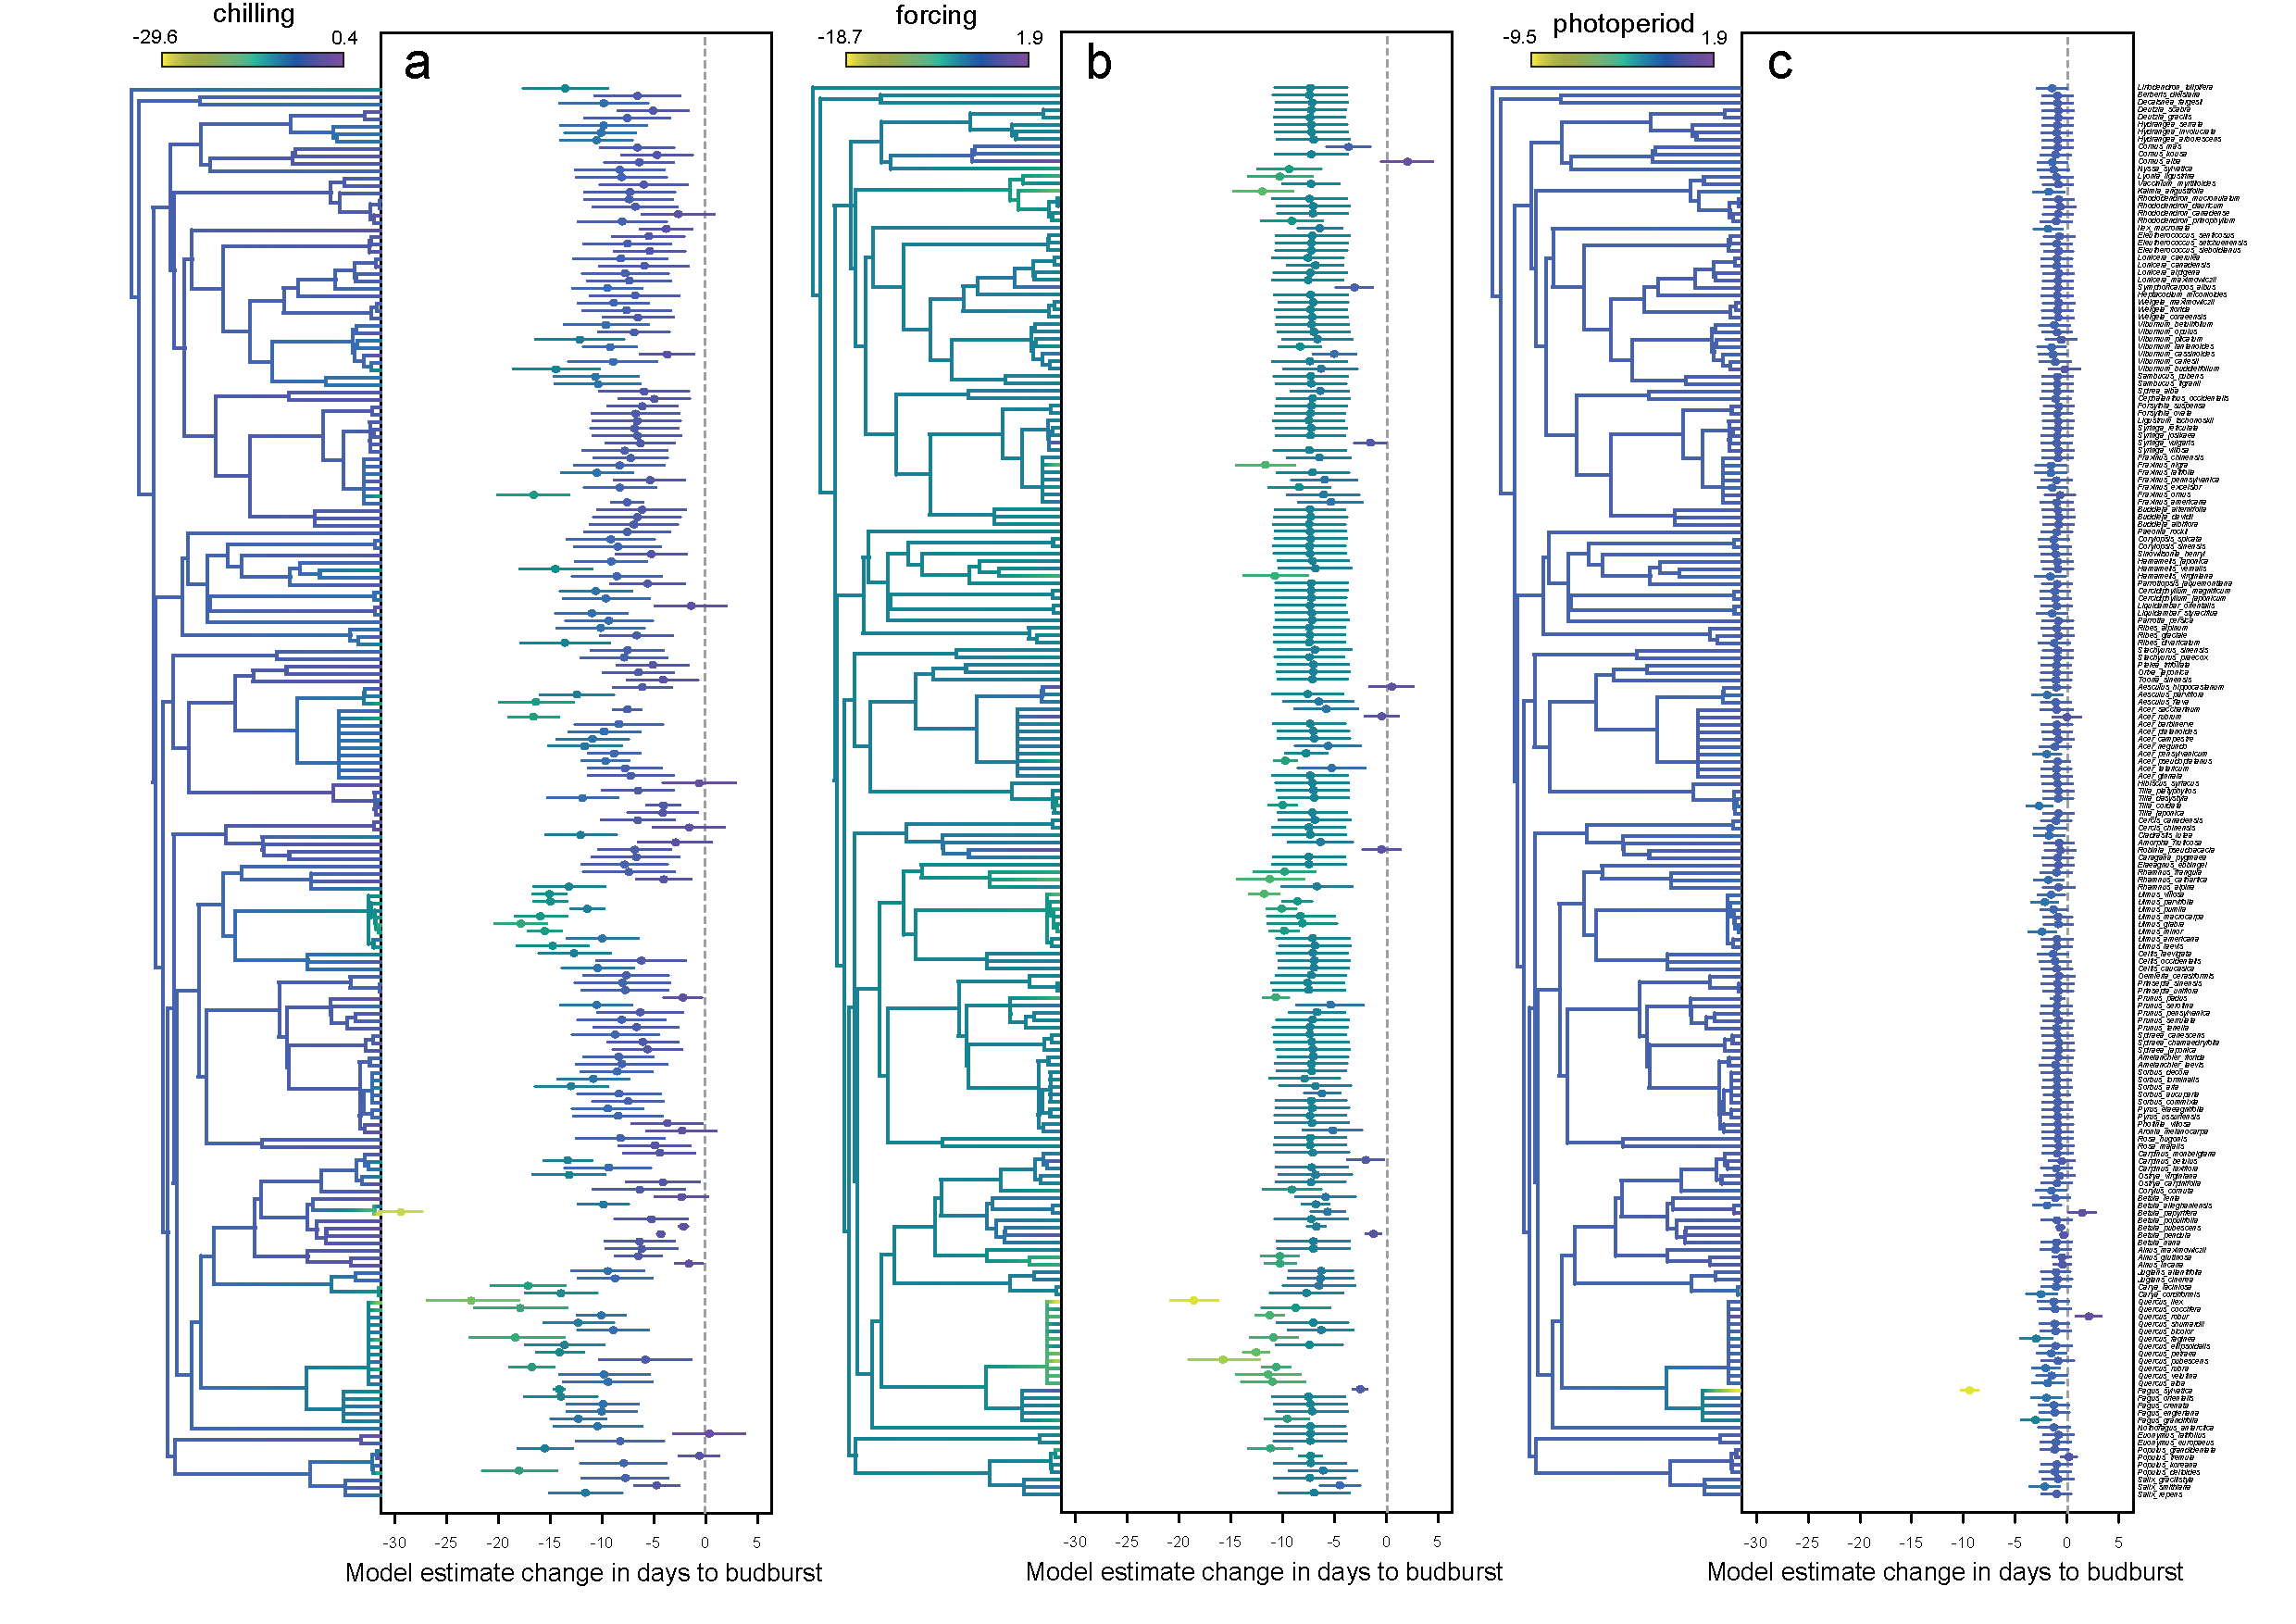
\includegraphics[width=16cm]{../../analyses/phylogeny/figures/FigSXX_ phylo_muplots191_lamb0.pdf}
  \caption{Non-phylogenetic phenological sensitivity to three environmental cues, chilling (a), forcing (b) and photoperiod (c) measured in change in days to budburst per standardized unit (z-transformation) of the cues across 191 tree species. Sensitivity estimates are computed by commonly used hierarchical model where phylogenetic distances are not accounted for ($\lambda$ = 0). The same phylogenetic tree is shown in each panel, colored acording to an estimation of ancestral character states, being the states at the tips the species' sensitivities to a cue. Species sensitivities are shown along with 50\% uncertainty Intervals in the diagrams. Note that the color scale varies in each panel. Total tree depth is 81. My.}
  \label{fig:suppmuplot_all} 
  \end{center}
\end{figure}

\clearpage
\begin{figure}
  \begin{center}
  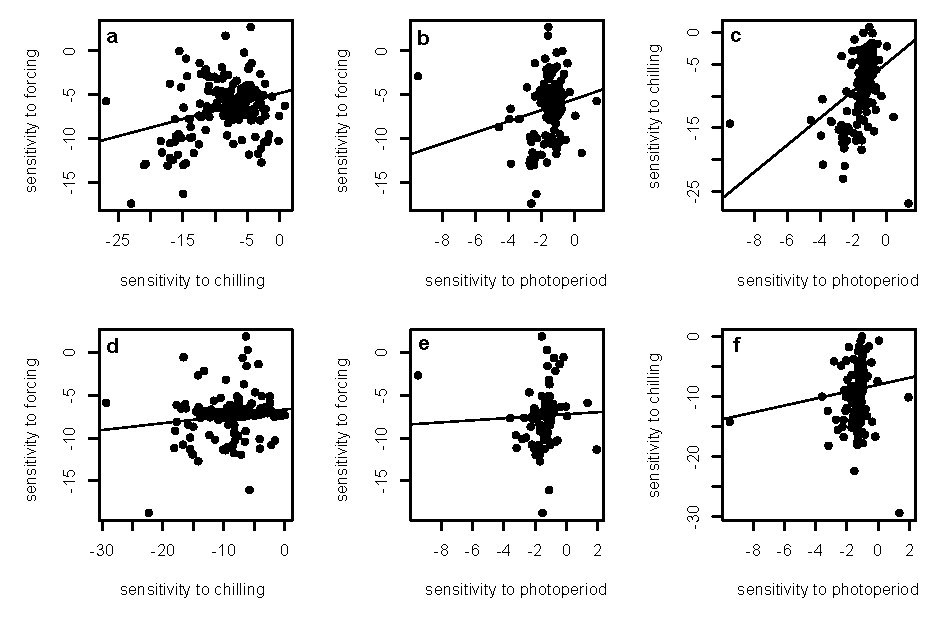
\includegraphics[width=16cm]{../../analyses/phylogeny/figures/FigSX_Sindromes_lamb_lamb0.pdf}
  \caption{Correlations among estimated sensitivities to the environmental cues comparing forcing vs. chilling (a,d), forcing vs. photoperiod (b,e) and chilling vs. photoperiod (c,f). Upper panels show correlations among estimated sensitivities by the phylogenetic model and lower panels show results for the non-phylogenetic model.}
  \label{fig:suppcorrelsens}
  \end{center}
\end{figure}

\clearpage
\begin{figure}
  \begin{center}
  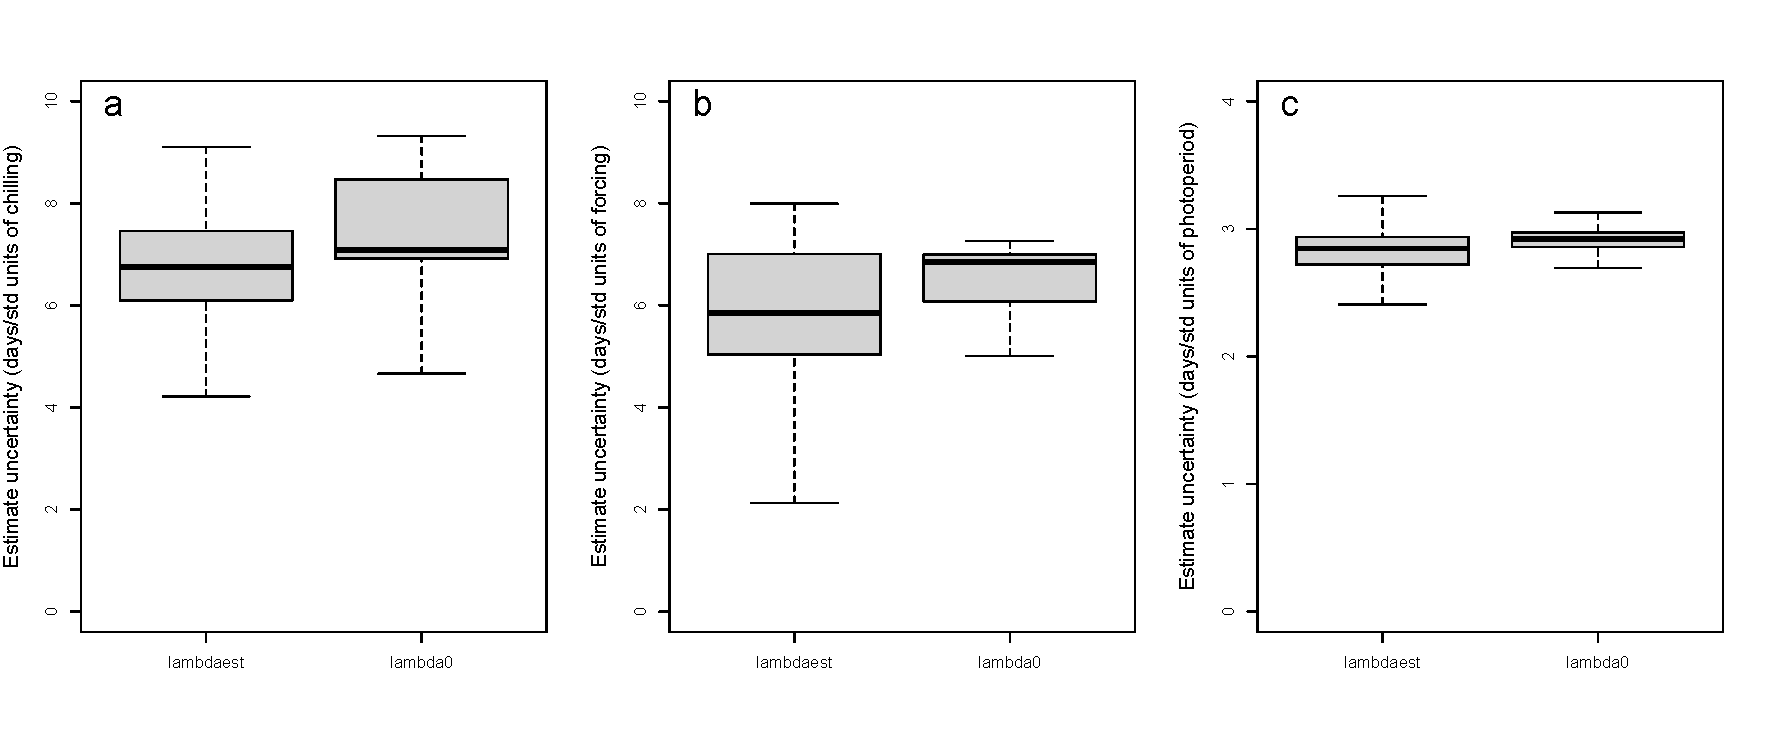
\includegraphics[width=16cm]{../../analyses/phylogeny/figures/FigSXXX_comparison_eachsps_uncertainty.pdf}
  \caption{Comparison of uncertainty around estimated sensitivities to chilling (a), forcing (b) and photoperiod (c) of individual species between the phylogenetic model with estimated $\lambda$ (lambdaest), and the non-phylogenetic model with $\lambda$ = 0 (lambda0). The non-phylogenetic model increases uncertainty.}
  \label{fig:suppuncertainties}
  \end{center}
\end{figure}

\clearpage
\begin{figure}
  \begin{center}
  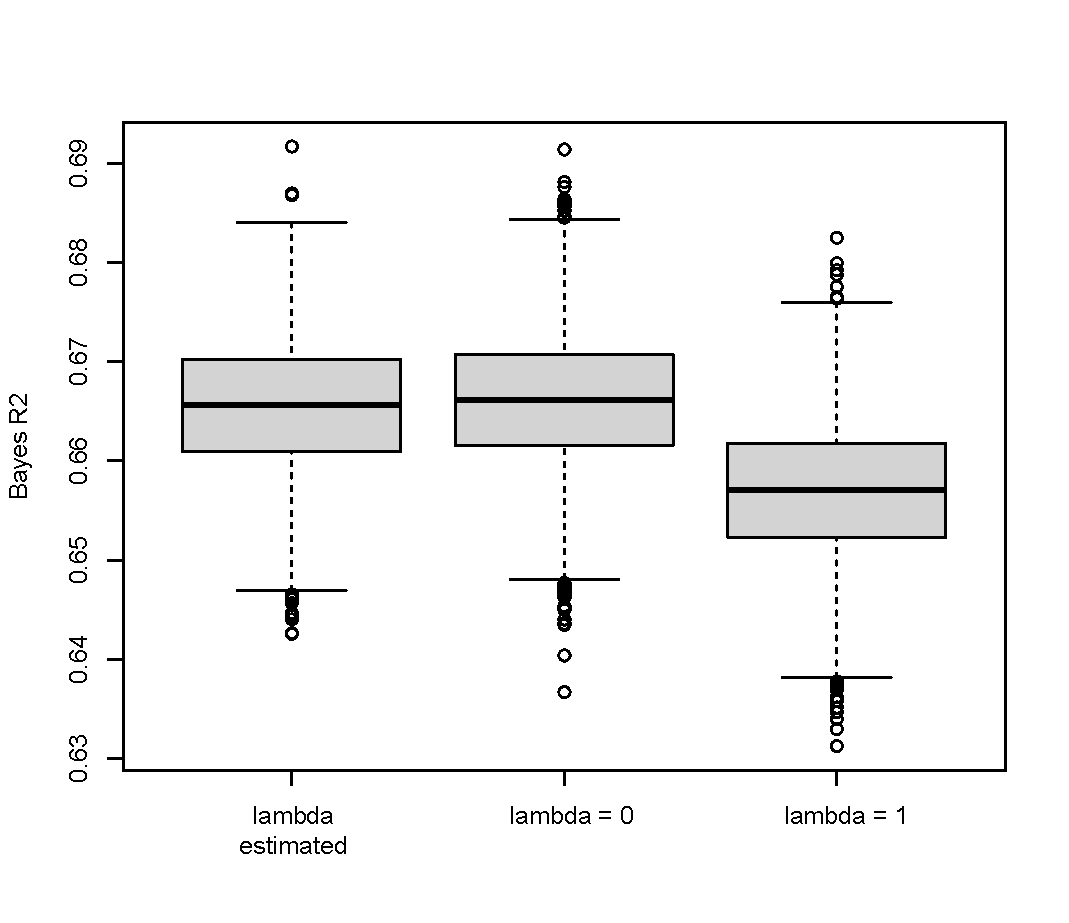
\includegraphics[width=16cm]{../../analyses/phylogeny/figures/Boxplot_bayesR2.pdf}
  \caption{Comparison of overall model accuracy as measured by Bayes \emph{R2} for the phylogenetic model (PMM) and the non-phylogenetic model (HMM). There are no differences in accuracy even if individual species estimates markedly differ between models.}
  \label{fig:accuracycomp}
  \end{center}
\end{figure}

\clearpage
\begin{figure}
  \begin{center}
  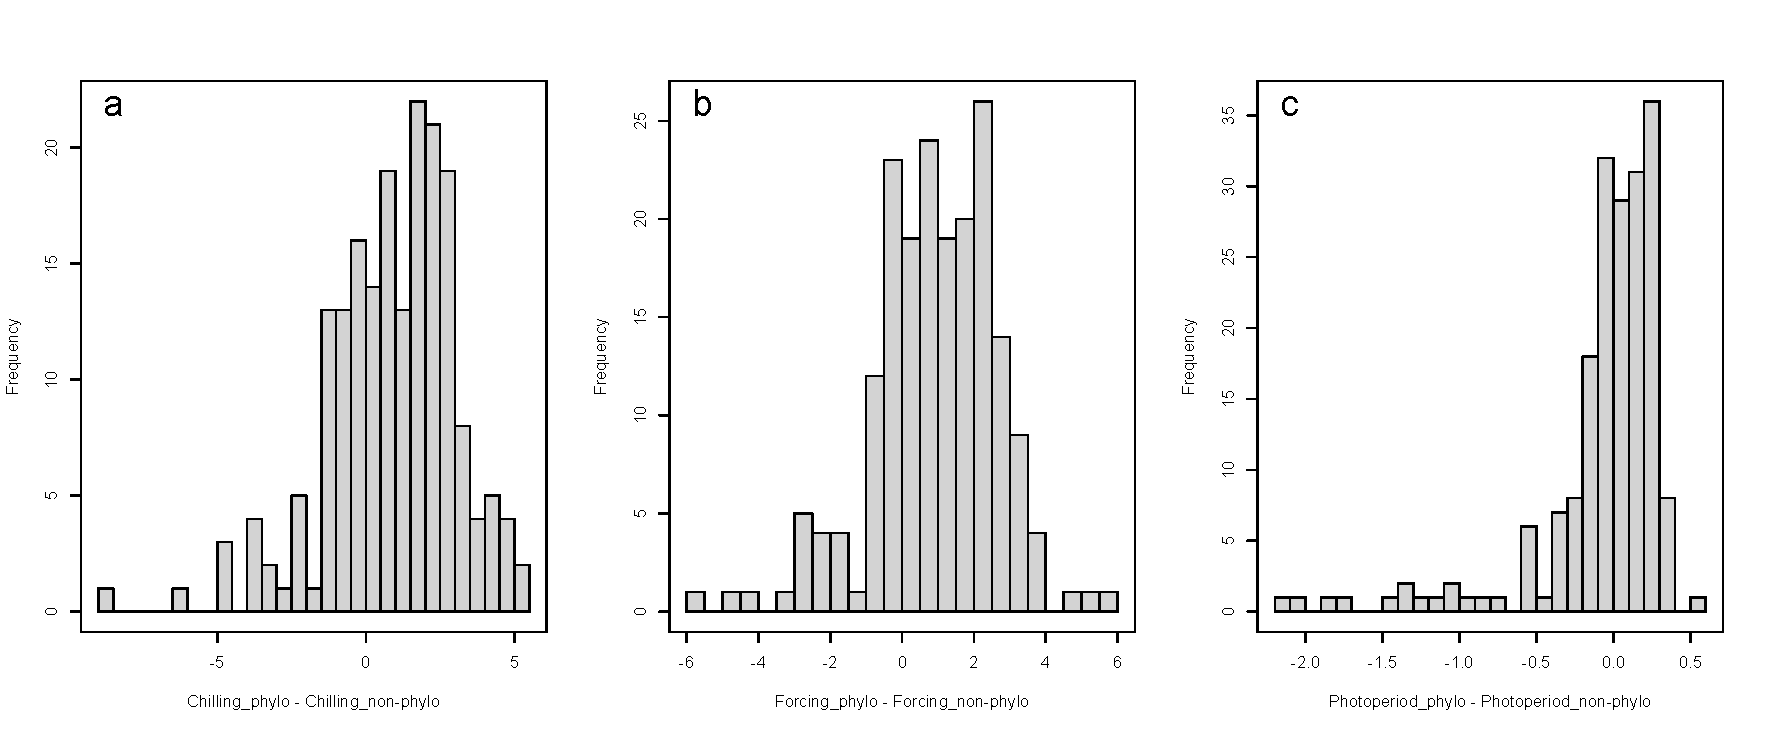
\includegraphics[width=14cm]{../../analyses/phylogeny/figures/FigSXX_bias_sens_phylo_nonphylo.pdf}
  \caption{Bias in estimation of sensitivity to chilling (a), forcing (b) and photoperiod (c). Histograms show the difference between the phylogenetic model with estimated $\lambda$ against the non-phylogenetic model with $\lambda$ = 0. Positive values indicate that sensitivities estimated by the non-phylogenetic model are smaller than those estimated by the phylogenetic model.}
  \label{fig:biasestimation}
  \end{center}
\end{figure}


\clearpage
\begin{figure}
  \begin{center}
  \includegraphics[width=16cm]{../../analyses/phylogeny/figures/Figsupp_forecasting_maps_pngnice.pdf}
  \caption{Maps comparing projections of phylogenetic (PMM) against non-phylogenetic (HMM) models into the European distributions of two overlapping species, one well represented in the dataset \emph{Betula pendula} (a) and one underrepresented \emph{Acer campestre} (b). The color scale shown in maps and histograms reflects budbreak differences between models where days are relative to start of forcing conditions, not calendar days.}
  \label{fig:pmmvshmm}
  \end{center}
\end{figure}


\clearpage
\begin{figure}
  \begin{center}
  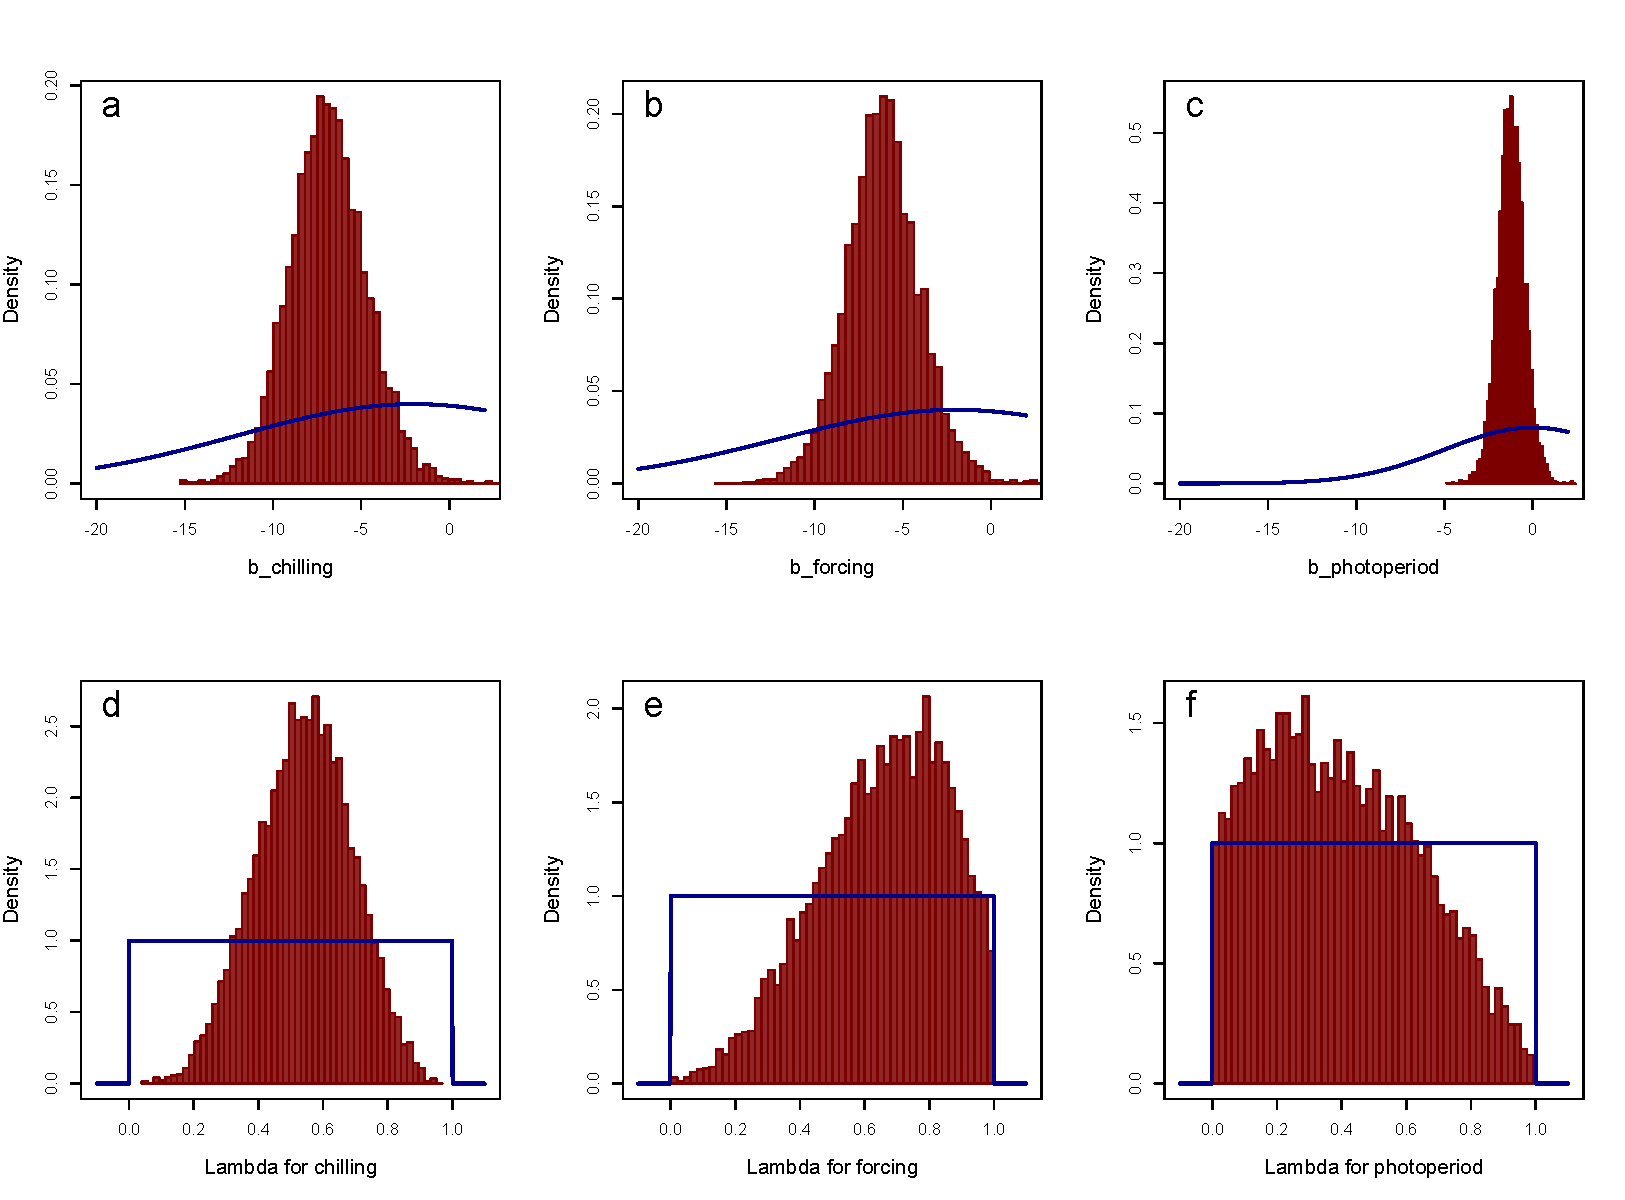
\includegraphics[width=14cm]{../../analyses/phylogeny/figures/FigSXX_marginal_plots_betas_lambda.pdf}
  \caption{Marginal plots contrasting the posterior distributions (in red) of estimated sensitivities to chilling (a), forcing (b) and photoperiod (c) against prior distributions (blue). Lower panels show marginal plots for the posterior distributions of phylogenetic parameter $\lambda$ fitted for chilling (d), forcing (e) and photoperiod (f). See \emph{Stan code} section below for details on prior and parameter specification of the models.}
  \label{fig:marginalplots}
  \end{center}
\end{figure}


\clearpage
\begin{figure}
  \begin{center}
  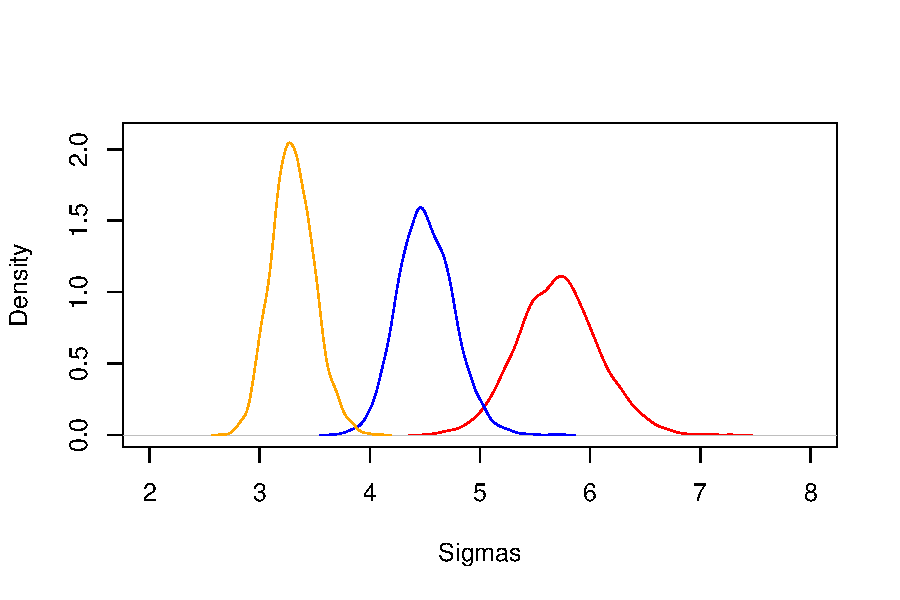
\includegraphics[width=14cm]{../../analyses/phylogeny/figures/burstmodelfigquick.pdf}
  \caption{Estimates of sigmas using our phylogenetic model and simulated data with responses to forcing and photoperiod generated from a delta model of evolution (fastBM in phytools package), with delta set to 2 for forcing and to 0.5 for photoperiod (intercept and chilling generated from lambda model with a lambda of 1).}
  \label{fig:burstmodels}
  \end{center}
\end{figure}


\clearpage
\section*{Stan code}
\begin{verbatim}

functions {
  matrix lambda_vcv(matrix vcv, real lambda, real sigma){
    matrix[rows(vcv),cols(vcv)] local_vcv; 
    local_vcv = vcv * lambda;
    for(i in 1:rows(local_vcv))
      local_vcv[i,i] = vcv[i,i];
      return(quad_form_diag(local_vcv, rep_vector(sigma, rows(vcv))));
  }
}

data {
  int<lower=1> N;
  int<lower=1> n_sp;
  int<lower=1, upper=n_sp> sp[N];
  vector[N] y; 		// response
  vector[N] x1; 	// predictor (forcing)
  vector[N] x2; 	// predictor (chilling)
  vector[N] x3; 	// predictor (photoperiod)
  matrix[n_sp,n_sp]Vphy;     // phylogeny
}

parameters {
  real<lower=0> sigma_y;    
  real<lower=0, upper=1> lam_interceptsa;       
  real<lower=0> sigma_interceptsa;
  real<lower=0, upper=1> lam_interceptsbf;       
  real<lower=0> sigma_interceptsbf;   
  real<lower=0, upper=1> lam_interceptsbc;       
  real<lower=0> sigma_interceptsbc; 
  real<lower=0, upper=1> lam_interceptsbp;       
  real<lower=0> sigma_interceptsbp; 
  vector[n_sp] b_force; // slope of forcing effect
  real b_zf;
  vector[n_sp] b_chill; // slope of chilling effect
  real b_zc;
  vector[n_sp] b_photo; // slope of photo effect
  real b_zp;
  vector[n_sp] a; // intercept
  real a_z;

}

model {
       real yhat[N];
       
        matrix[n_sp,n_sp] vcv_a;     // phylogeny
        matrix[n_sp,n_sp] vcv_bf;     // phylogeny
        matrix[n_sp,n_sp] vcv_bc;     // phylogeny
        matrix[n_sp,n_sp] vcv_bp;     // phylogeny

       
       	for(i in 1:N){
            yhat[i] = 
	      a[sp[i]] + b_force[sp[i]] * x1[i] + b_chill[sp[i]] * x2[i] + b_photo[sp[i]] * x3[i];
			     	}
			     	
	vcv_a = cholesky_decompose(lambda_vcv(Vphy, lam_interceptsa, sigma_interceptsa));
  vcv_bf = cholesky_decompose(lambda_vcv(Vphy, lam_interceptsbf, sigma_interceptsbf));
  vcv_bc = cholesky_decompose(lambda_vcv(Vphy, lam_interceptsbc, sigma_interceptsbc));
  vcv_bp = cholesky_decompose(lambda_vcv(Vphy, lam_interceptsbp, sigma_interceptsbp));


  a ~ multi_normal_cholesky(rep_vector(a_z,n_sp), vcv_a); 
  b_force ~ multi_normal_cholesky(rep_vector(b_zf,n_sp), vcv_bf); 
  b_chill ~ multi_normal_cholesky(rep_vector(b_zc,n_sp), vcv_bc);
  b_photo ~ multi_normal_cholesky(rep_vector(b_zp,n_sp),vcv_bp);
  
  y ~ normal(yhat, sigma_y);

    a_z ~ normal(30, 10); // prior
    b_zf ~ normal(-2, 10); //  prior 
    b_zc ~ normal(-2, 10); //  prior
    b_zp ~ normal(0, 5); //  prior

    lam_interceptsa ~ beta(1, 1);
    lam_interceptsbf ~ beta(1, 1);
    lam_interceptsbc~ beta(1, 1);
    lam_interceptsbp ~ beta(1, 1);

    sigma_interceptsa ~ normal(30, 20);
    sigma_interceptsbf ~ normal(1, 5);
    sigma_interceptsbc ~ normal(1, 5);
    sigma_interceptsbp ~ normal(1, 5);
    
    sigma_y ~ normal(10, 10); // prior
  
}


\end{verbatim}



\end{document}
